% !TeX spellcheck = <none>

%contains all the imports and configurations 

\documentclass[10pt,a4paper]{report}
\usepackage[a4paper, left=2cm, right=2cm, top=2cm, bottom=2cm]{geometry}
\usepackage[utf8]{inputenc}		%utf8 allows also for umlauts
\usepackage[english]{babel}
\usepackage{amsmath}

%Declare new math operators with amsmath:

%atan2 function
\DeclareMathOperator{\atantwo}{atan2}
\DeclareMathOperator{\arctantwo}{arctan2}
\DeclareMathOperator{\acos}{acos}

%Decalre new math font:
\usepackage{mathrsfs}


\usepackage{amsfonts}
\usepackage{amssymb}
\usepackage{graphicx}	%for importing images
\graphicspath{ {./images/} {../GeneratedPlots/} }
\usepackage{gensymb}
\usepackage{siunitx}
%\usepackage[numbered,framed]{matlab-prettifier}
\usepackage{float}
\usepackage[usenames,dvipsnames]{color} % color text
\definecolor{mygreen}{RGB}{28,172,0} % color values Red, Green, Blue
\definecolor{mylilas}{RGB}{170,55,241}

%coloured text
\usepackage{xcolor} %\textcolor{blue}{This is a sample text in blue.}

\usepackage{listings}
\usepackage{alphalph}

\usepackage{breqn} %automatic linebreaking math environment
%insert after all math stuff e.g. amsmath, amssymb mathpazo... is imported

%insert external pdf pages in document
\usepackage{pdfpages} 
% http://texdoc.net/texmf-dist/doc/latex/pdfpages/pdfpages.pdf

%Bibliography settings
\usepackage[citestyle = numeric, bibstyle=numeric]{biblatex} %style =apa %citestyle = numeric, style=numeric, bibstyle = numeric
\addbibresource{References.bib}    

% for including current date into document
\usepackage[ddmmyyyy]{datetime}

%Give captions to items that normally don't have any
\usepackage{caption} 
%use as:
%\DeclareCaptionType{exam}[Example][List of Examples]
%\listofexams
%\begin{enumerate}
%	\item First item.
%	\item Second item.
%	\item Third item.
%	\captionof{exam}{This is a very important list.}
%\end{enumerate}

%For making an appendix
\usepackage[toc,page]{appendix}

% \usepackage[table,xcdraw]{xcolor}

%line drawing in array or tabular
%\usepackage{arydshln} %here used for mimicing matrices in array with dashed lines
%Doesn't work as intended

%Matrix options for dotted lines, etc. etc...
\usepackage{nicematrix} % here used for makin g arrays with dashed separator lines
%http://ctan.math.washington.edu/tex-archive/macros/latex/contrib/nicematrix/nicematrix.pdf

\usepackage{enumitem}
\usepackage{multicol}%try it out!





%acronym package (needs an acronym chapter)
%\usepackage{acronym}
%\usepackage{acro}	%Alternative, more elaborate package for acronyms
%\acsetup{hyperref = true, only-used = true, sort = true,  }

\DeclareAcronym{HAN}{short = HAN , long = Hogeschool van Arnhem en Nijmegen }
\DeclareAcronym{SPC}{short = SPC , long = Smart Production Cell }
\DeclareAcronym{PC}{short = PC , long = Personal Computer }
\DeclareAcronym{DOF}{short DOF = , long = Degree of Freedom }






%\begin{acronym}[Bash]

%	\acro{HAN}{Hogeschool van Arnhem en Nijmegen}
%	\acro{SPC}{Smart Production Cell}
%	\acro{DOF}{degrees of freedom}
%	\acro{FRC}{Fibre Reinforced Composites}
%	\acro{DH}{Denavit-Hartenberg}
%	\acro{IOT}{Internet Of Things}
%	\acro{FHEM}{Freundliche Hausautomation und Energie-Messung \cite{FHEM}}
%	\acro{NFC}{Near-field communication}
%	\acro{IPKW}{Industrial Park Kleevse Waard}
%	\acro{NFC}{Near Field Communication}
%	\acro{ROS}{Robot Operating System}
%	\acro{GUI}{Graphical User Interface}
%	\acro{EOAT}{End Of Arm Tooling}
%	\acro{PL}{Production Line}
%	\acro{ETCS}{European Train Control System}
%	\acro{DT}{Digital Twin}
%	\acro{eq}{equation}
%	\acro{DCS}{Dual Check Safety}
%	\acro{DDS}{Data Distribution System}
%	\acro{fig}{figure}
%	\acro{sect}{section}
%	\acro{OS}{Operating System}
%\end{acronym}


%import PDF pages
\usepackage{pdfpages}
%To include all the pages in the PDF file:
%\includepdf[pages=-]{myfile.pdf}
%To include just the first page of a PDF:
%\includepdf[pages={1}]{myfile.pdf}

%Start new chapter on same page to avaoid big spaces
\usepackage{etoolbox}
\makeatletter
\patchcmd{\chapter}{\if@openright\cleardoublepage\else\clearpage\fi}{}{}{}
\makeatother

% Incluse subsubsection in Toc
\setcounter{tocdepth}{2}
\setcounter{secnumdepth}{3}

 %Wildcard for Signature line
\newcommand*\wildcard[2][6cm]{\vspace*{0.5cm}\parbox{#1}{\hrulefill\par#2}}

%A truly random package
\usepackage{lipsum} %random text

%If custom headers are needed
%\usepackage{fancyhdr}
%
%\pagestyle{fancy}
%\fancyhf{}
%\rhead{Overleaf}
%\lhead{Guides and tutorials}
%\rfoot{Page \thepage}

%for left, center or right aligning figures
\usepackage[export]{adjustbox}
%https://tex.stackexchange.com/questions/91566/syntax-similar-to-centering-for-right-and-left

%Remove word "chapter" but leave numbering
\makeatletter
\renewcommand{\@makechapterhead}[1]{%
	\vspace*{50 pt}%
	{\setlength{\parindent}{0pt} \raggedright \normalfont
		\bfseries\Huge\thechapter.\ #1
		\par\nobreak\vspace{40 pt}}}
\makeatother

%Add line below chapter title and minimze space when text starts
%\usepackage[]{titlesec}
%\titleformat{\chapter}[hang]{\huge\sffamily\bfseries}{}{0pt}{}[\hrule\vspace*{-23pt}] 

%no indentation for paragraphs
\setlength{\parindent}{0cm}

\usepackage{hyperref} %Load last as it can cause trouble with other packages. For Hyperlink https://de.wikibooks.org/wiki/LaTeX-W%C3%B6rterbuch:_hyperref
\hypersetup{
	colorlinks=true,
	linkcolor=blue,
	filecolor=magenta,      
	urlcolor=cyan,
}
\urlstyle{same} %The default is equivalent to \urlstyle{tt}; with \urlstyle{rm} and \urlstyle{sf} the font will be the roman or sans serif upright font. With \urlstyle{same} the current font will be used.

\usepackage{cleveref} %multi reference with \cref{x,y}
% needs to be loaded after hyperref 

%Define \fulref command for nice cross referencing in document with hyperlinks:
\newcommand*{\fullref}[1]{\hyperref[{#1}]{\autoref*{#1} \nameref*{#1}}} 
%How to use: see
% https://tex.stackexchange.com/questions/121865/nameref-how-to-display-section-name-and-its-number

%Making a Glossary
%\usepackage{glossaries}
\usepackage[acronyms,shortcuts,symbols,xindy,nonumberlist]{glossaries-extra}%,numberedsection
%\usepackage[style=long,toc,automake]{glossaries}
%https://en.wikibooks.org/wiki/LaTeX/Glossary
%http://tug.ctan.org/macros/latex/contrib/glossaries/glossariesbegin.pdf
\setabbreviationstyle[acronym]{long-short}

	\newacronym{DCS}{DCS}{Dual Check Safety}
	\newacronym{DDS}{DDS}{Data Distribution System}
	\newacronym{DH}{DH}{Denavit-Hartenberg}
	\newacronym{DOF}{DOF}{degrees of freedom}
	\newacronym{DT}{DT}{Digital Twin}
	%E
	\newacronym{EOAT}{EOAT}{End Of Arm Tooling}
	\newacronym{eq}{eq}{equation}
	\newacronym{ETCS}{ETCS}{European Train Control System}
	%F
	\newacronym{FHEM}{FHEM}{Freundliche Hausautomation und Energie-Messung \cite{FHEM}}
	\newacronym{fig}{fig}{figure}
	\newacronym{FRC}{FRC}{Fibre Reinforced Composites}
	%G
	\newacronym{GUI}{GUI}{Graphical User Interface}
	%H
	\newacronym{HAN}{HAN}{Hogeschool van Arnhem en Nijmegen}
	%I
	\newacronym{IOT}{IOT}{Internet Of Things}
	\newacronym{IPKW}{IPKW}{Industrial Park Kleevse Waard}
	%J
	%K
	%L
	%M
	%N
	\newacronym{NFC}{NFC}{Near-field communication}
	%O
	\newacronym{OS}{OS}{Operating System}
	%P
	\newacronym{PC}{PC}{Personal Computer}
	\newacronym{PL}{PL}{Production Line}
	%Q
	%R
	\newacronym{ROS}{ROS}{Robot Operating System}
	%S
	\newacronym{sect}{sect}{section}
	\newacronym{SPC}{SPC}{Smart Production Cell}
%Glossary entries listed here


\newglossaryentry{numSol}{
	name={Numerical Solution},
	description={Originally the term numerical solution describes a solution given in terms of numbers instead of an explicit closed form expression. In this work, the term "numerical solution" refers to numerical, iterative methods for solving the inverse kinematics problem by using a sequence of steps leading to incrementally better solutions for the joint angles. Examples for these methdods are the jacobian inversion method, the optimization based method cyclic coordinate descent as shown by Lukas Barinka \cite{InvkinMeth_Lukas}. 
}}

\newglossaryentry{forwKin}{name={forward kinematics},description={Forward kinematics describes the position of the endpoint of a kinematic chain in the operational space by the kinematic equations with the joint variables as input. The non-linear kinematic equations map the joint parameters to the configuration of the robot system. This results in a pure geometrical description of motion by means of position, orientation, and their time derivatives.}}

\newglossaryentry{joints}{name={joint},description={A joint is a connection between two links that allows for movement within certain contstraints. }}

\newglossaryentry{link}{name={link},description={A link is a rigid body, defining the
		spatial relationship between two following axes. Links can be rotated or translated by joints, but don't deform themselves.}}
%\glsxtrnewsymbol[description={position}]{x}{\ensuremath{x}}
%\glsxtrnewsymbol[description={velocity}]{v}{\ensuremath{v}}
%\glsxtrnewsymbol[description={acceleration}]{a}{\ensuremath{a}}
%\glsxtrnewsymbol[description={time}]{t}{\ensuremath{t}}
%\glsxtrnewsymbol[description={force}]{F}{\ensuremath{F}}

%\glsxtrnewsymbol[description={}]{}{\ensuremath{}}

\glsxtrnewsymbol[description={joint iteration variable}]{n}{\ensuremath{n}}
\glsxtrnewsymbol[description={link iteration variable}]{i}{\ensuremath{i}}
\glsxtrnewsymbol[description={Number of joints}]{N}{\ensuremath{N}}
\glsxtrnewsymbol[description={Number of links}]{I}{\ensuremath{I}}

\glsxtrnewsymbol[description={local coordinate frame x -axis}]{x_i}{\ensuremath{x_i}}
\glsxtrnewsymbol[description={local coordinate frame y -axis}]{y_i}{\ensuremath{y_i}}
\glsxtrnewsymbol[description={local coordinate frame z -axis}]{z_i}{\ensuremath{z_i}}

\glsxtrnewsymbol[description={rotation around the $x_i$-axis}]{alpha_i}{\ensuremath{\alpha_i}}
\glsxtrnewsymbol[description={translation along $x_i$-axis}]{a_i}{\ensuremath{a_i}}
\glsxtrnewsymbol[description={translation along $z_i$-axis}]{d_i}{\ensuremath{d_i}}
\glsxtrnewsymbol[description=rotation around $z_i$-axis{}]{theta_i}{\ensuremath{\theta_i}}

\glsxtrnewsymbol[description={Vector}]{v}{\ensuremath{v}}

\glsxtrnewsymbol[description={normal vector}]{n_xyz}{\ensuremath{n_{xyz}}}
\glsxtrnewsymbol[description={orientation vector}]{o_xyz}{\ensuremath{o_{xyz}}}
\glsxtrnewsymbol[description={approach vector}]{a_xyz}{\ensuremath{a_{xyz}}}
\glsxtrnewsymbol[description={position vector}]{p_xyz}{\ensuremath{p_{xyz}}}

\glsxtrnewsymbol[description={x-position within frame}]{x}{\ensuremath{x}}
\glsxtrnewsymbol[description={y-position within frame}]{y}{\ensuremath{y}}
\glsxtrnewsymbol[description={z-position within frame}]{z}{\ensuremath{z}}
\glsxtrnewsymbol[description={rotation around x}]{alpha}{\ensuremath{\alpha}}
\glsxtrnewsymbol[description={rotation around y}]{beta}{\ensuremath{\beta}}
\glsxtrnewsymbol[description={rotation around z}]{gamma}{\ensuremath{\gamma}}

\glsxtrnewsymbol[description={Transformation matrix}]{T}{\ensuremath{T}}
\glsxtrnewsymbol[description={Rotation matrix}]{R}{\ensuremath{R}}

\glsxtrnewsymbol[description={$\sin(\theta_i)$}]{s_i}{\ensuremath{s_i}}
\glsxtrnewsymbol[description={$\cos(\theta_i)$}]{c_i}{\ensuremath{c_i}}

\glsxtrnewsymbol[description={Position with orientation in euclidean space $p=(x,y,z,\alpha,\beta,\gamma)$}]{p}{\ensuremath{p}}
\glsxtrnewsymbol[description={joint angles in joinet space $q=(q_1, q_2, q_3, q_4, q_5, q_6)$ }]{q}{\ensuremath{q}}

\glsxtrnewsymbol[description={Jacobian matrix}]{J}{\ensuremath{J}}
\glsxtrnewsymbol[description={Joint-space inertia matrix}]{M}{\ensuremath{M}}
\glsxtrnewsymbol[description={Coriolis and centripetal coupling matrix}]{C}{\ensuremath{C}}
\glsxtrnewsymbol[description={force}]{F}{\ensuremath{F}}
\glsxtrnewsymbol[description={Gravity loading}]{G}{\ensuremath{G}}
\glsxtrnewsymbol[description={Wrench applied at the end effector}]{W}{\ensuremath{W}}

\glsxtrnewsymbol[description={generalized actuator forces}]{Q}{\ensuremath{Q}}
\glsxtrnewsymbol[description={actuator torque}]{Upsilon}{\ensuremath{\Upsilon}}

\glsxtrnewsymbol[description={Lagrangian}]{L}{\ensuremath{L}}
\glsxtrnewsymbol[description={Kinetic Energy}]{KinEner}{\ensuremath{T(q,\dot{q})}}
\glsxtrnewsymbol[description={Potential energy}]{PotEner}{\ensuremath{V(q)}}

\glsxtrnewsymbol[description={Innertia Matrix}]{InertiaMatr}{\ensuremath{\mathcal{I}}}

\glsxtrnewsymbol[description={link mass}]{m}{\ensuremath{m}}
\glsxtrnewsymbol[description={width}]{w}{\ensuremath{w}}
\glsxtrnewsymbol[description={height}]{h}{\ensuremath{h}}
\glsxtrnewsymbol[description={length}]{l}{\ensuremath{k}}
\glsxtrnewsymbol[description={Christoffel symbol}]{Christoffel}{\ensuremath{\Gamma_{...}}}


%\glsxtrnewsymbol[description={}]{}{\ensuremath{}}

%Note: Don't use dots in filenames, as this can lead to errors, e.g. with glossary package. Here the filename is cut after the dot, so wrong filenames are used for processing and will lead to errors.

%remove clear page before printglossary
\renewcommand*{\glsclearpage}{}



\makeglossaries
%\makenoidxglossaries



%Include list of figures and list of tables in TOC
\usepackage{tocbibind}


%Set some things clear 
\newcommand{\HANSupervisor}{Wesselingh Ellen}
\newcommand{\CompanySupervisor}{Nguyen Trung}
\newcommand{\AdditionalSupervisor}{Jeltsema Dimitri}
\author{Karl Wallkum}

%% Preamble 
%Deactivate before Distribution!!



\begin{document}
	\pagenumbering{roman}
		
	\input{Frontpage/titlepage}
	\begin{figure}[H]
	\centering
	\includegraphics[
	width=1\linewidth,
	height=\paperheight,
	keepaspectratio,
	]{fanuc210_corner_cut}
	\caption{FANUC R-2000iC/210F 6-axis industrial robot arm}
	\label{fig:fanuc210}
\end{figure}
\pagestyle{empty}

	\cleardoublepage
	
	% !TeX spellcheck = <none>
%testtest
%\chapter{Summary}


	
	\newpage
	\tableofcontents
	
	\thispagestyle{empty}
	\clearpage
	\pagenumbering{arabic}
	
	%\section*{title}
The goal of this assignment is to ..\\
textextextext\\

\begin{table}[h]
	\centering
	\begin{tabular}{|l c l|}
		\hline
			&	&	\\
			&	&	\\
			&	&	\\
			&	&	\\
		\hline
	\end{tabular}
	\caption{caption}
	\label{Tab:table1}
\end{table}
%
textext as seen in Table \ref{Tab:table1} textextext.\\

\begin{figure}[H]
	\centering
	\includegraphics[
	width=0.8\linewidth,
	height=\paperheight,
	keepaspectratio,
	]{testimage}
	\caption{Y vs X}
	\label{fig:image1}
\end{figure}

\newpage
	
	\chapter{Abstract}
%~150Words

This work aims to integrate a FANUC 210F 6 axis industrial robot arm  into an experimental production line. 
As this production line is set in a research environment, gaining a deeper understanding of all involved systems is desired.\\
\\
The dynamic behaviour of a physical system is best expressed with an analytical model.
In order to control a robot arm, a kinematic model needs to be created. With this model, a control algorithm can be derived.\\
\\
The objective of this thesis is to derive the complete inverse kinematic model of a 6 \ac{DOF} robotic arm analytically. For an exact numerical simulation of the device most steps are laid out theoretically and difficulties in the practical implementation are described.
Additionally for follow up projects this work also contains a quick start guide and a safety manual for the robot in this setting .
Finally to contribute to current research, twinning specifications will be defined.


%See: https://www.sfu.ca/~jcnesbit/HowToWriteAbstract.htm
%
%%What is an Abstract?
%
%The abstract is an important component of your thesis. Presented at the beginning of the thesis, it is likely the first substantive description of your work read by an external examiner. You should view it as an opportunity to set accurate expectations.
%The abstract is a summary of the whole thesis. It presents all the major elements of your work in a highly condensed form.
%An abstract often functions, together with the thesis title, as a stand-alone text. Abstracts appear, absent the full text of the thesis, in bibliographic indexes such as PsycInfo. They may also be presented in announcements of the thesis examination. Most readers who encounter your abstract in a bibliographic database or receive an email announcing your research presentation will never retrieve the full text or attend the presentation.
%An abstract is not merely an introduction in the sense of a preface, preamble, or advance organizer that prepares the reader for the thesis. In addition to that function, it must be capable of substituting for the whole thesis when there is insufficient time and space for the full text. 
%
%
%%Size and Structure
%
%Currently, the maximum sizes for abstracts submitted to Canada's National Archive are 150 words (Masters thesis) and 350 words (Doctoral dissertation)
%The structure of the abstract should mirror the structure of the whole thesis, and should represent all its major elements.
%%For example, if your thesis has five chapters (introduction, literature review, methodology, results, conclusion), there should be one or more sentences assigned to summarize each chapter. 
%
%
%%Clearly Specify Your Research Questions
%
%As in the thesis itself, your research questions are critical in ensuring that the abstract is coherent and logically structured. They form the skeleton to which other elements adhere.
%They should be presented near the beginning of the abstract.
%There is only room for one to three questions. If there are more than three major research questions in your thesis, you should consider restructuring them by reducing some to subsidiary status. 
%
%Don't Forget the Results
%
%The most common error in abstracts is failure to present results.
%The primary function of your thesis (and by extension your abstract) is not to tell readers what you did, it is to tell them what you discovered. Other information, such as the account of your research methods, is needed mainly to back the claims you make about your results.
%Approximately the last half of the abstract should be dedicated to summarizing and interpreting your results. 


%%Example and Tips: https://www.scribbr.de/aufbau-und-gliederung/abstract-schreiben/







	
	% !TeX spellcheck = <none>
%testtest
\section{Preface}
%Checklist Preface: https://www.scribbr.com/dissertation/preface-dissertation/

\paragraph{Definition of a Robot}
%% definition/clickbait
Robots \cite{robotDef} can be defined as programmable movement automatons \cite{automatonDef} that can perform tasks without human supervision and can be taught at least repetitive tasks. 
Increasingly, also ways to sense their surroundings are added and improve their movements according to the situation \cite{robotDef2}. 
These sensors are placed additionally to the standard feedback-control sensors like pulse encoders. % at their axes to feedback control their endpoint position accuracy. 
%system supervision - robotic system - 
% A robot is defined as a programmable movement automaton, with the ability to perform tasks without human supervision. Not only can the robot be taught repetitive tasks, that it can execute with pulse encoders at their axes. it can as well sense its surroundings and on the basis of that information improve movements accordingly. 
% go to old from new! Go from general to specific Don't jump from general to specific to examples, don't mix it because reader has then to do all the work. and show that you are not only able to understand concepts, but are able to 1) present them in a coherent way and (later) critique them. chronology
\medskip


\paragraph{Origin of Robots}
The origin of Robots is well documented in "Robotics, Vision and Control: Fundamental Algorithms in MATLAB" by Peter Corke \cite{CorkeRoboticVisionControl}:
%From Corce Robotics Toolbox: (Refactor!)
"The term robot first appeared in a 1920 Czech science fiction play Rossum’s Universal Robots” by Karel .apek (pronounced Chapek). 
The term was coined by his brother Josef, and in the Czech language means serf labor but colloquially means hardwork or drudgery. 
The robots in the play were artificial people or androids and as in so many robot stories that follow this one, the robots rebel and it ends badly for humanity. 
Isaac Asimov’s robot series, comprising many books and short stories written between 1950 and 1985, explored issues of human and robot interaction and morality. 
The robots in these stories are equipped with “positronic brains” in which the “Three laws of robotics” are encoded. These stories have influenced subsequent books and movies which in turn have shaped the public perception of what robots are. 
The mid twentieth century also saw the advent of the field of cybernetics  – an uncommon term today but then an exciting science at the frontiers of understanding life and creating intelligent machines.
The first patent for what we would now consider a robot was filed in 1954 by George C. Devol and issued in 1961. 
The device comprised a mechanical arm with a gripper that was mounted on a track and the sequence of motions was encoded as magnetic patterns stored on a rotating drum. 
The first robotics company, Unimation, was founded by Devol and Joseph Engelberger in 1956 and their first industrial robot shown in Fig. \ref{fig:unimate} was installed in 1961. \cite{CorkeRoboticVisionControl}
%(Unimation) (Get picture from children book)
\medskip



\paragraph{Simple robots}
%% simple robots
I have started working with robots and robotic systems in my bachelor studies. 
As a starting engineer, I was exploring the possibilities of automated manufacturing with CNC mills and 3D printers. 
These were very simplistic robotic systems based on a feedforward control with stepper motors for position control. 
For starting a production process, these devices had to be half automatically calibrated and the position and orientation needed to be taught by pointing the drill/printing head to the markerpoints. 
As no feedback control is usually available on these devices, loss of step control and other errors are possible and can go unnoticed until the end of production, when the part is inspected.
\medskip


\paragraph{Current Robots}
%% current robots
Highly developed automated platforms like the Fanuc 210F have feedback-sensors and -control for point to point as well as tracking motion, computer vision as seen on the deltarobot, digital and analog I/O,  builtin- safety like the \ac{DCS} motion safety system and high speed fieldbus connectivity like Profient.
With a teach pendant, these Robots can be configured and programmed. Alternatively \ac{PC}-based proprietary manufacturer-specific software with a model based test cell can be used to program the robot. 
\medskip

\paragraph{Future robots}
%% future robot (envisioned)
To compete in the future developements of "Smart Manufacturing", "the Smart Cell  project investigates on an automated production cell for the realization of structural composite components which must be produced in large scale or mass produced" (see \cite{SPCWebsite}, Smart-Cell project description). 
Besides research in materials and production, the automation environment system is of interest for this research.
To manage the interaction between material but also the machines among each other, a \ac{DDS} couples the subsystems as a middlware as seen in \ac{fig}. \ref{fig:SmartCellDDS}. A middleware is "glue code" that helps to interface systems with each other to exchange commands and data to use it as a single robotic system. 
\ac{ROS} is a proposed middleware to model, simulate, and control the production line as a homogenious distributed system. 
Besides the classical publish subscribe  pattern to simplify network programming, \ac{ROS} provides an ecosystem of interchangeable nodes and drivers to provide a wide codebase for complex tasks.
\medskip
\begin{figure}[H]
	\includegraphics[
	width=0.95\linewidth,
	center,
	keepaspectratio,
	]{SmartCellDDS}
	\caption{\ac{DDS} as central information exchange platform}
	\label{fig:SmartCellDDS}
\end{figure}

%What are keywords for each of the paragraphs? e.g. HUMAN supervision, robotic Systems, etc..
%Use strong Verbs!
%signalwords
%

	\chapter*{Acknowledgements}

I want to thank everyone who has helped me with this thesis work. It was a great learning experience for me.\\
\\
First of all, I would like to thank Peter Verschut, the project manager at SPC, who has made this project possible. By providing the SPC lab at MIC and letting me do experiments with the machines, I could get a lot of practical experience with the Fanuc210F and other machines. Also he connected me with experts in the field so I could make contacts for further work in the field of robotics. \\
\\
Dimitri Jeltsema gave me a good hint how to model and control the robot based on the content of his lectures. Besides that, Ellen Wesselingh and Trung Nguyen have given me great advice on the writing and modelling of the robot. Without your guidance this journey would have been a lot harder. Your critical questioning and pushing in the right direction have helped me a lot. Thank you for your patience and effort. \\
\\
Peter Corke has made the modelling and control of the robot arm a lot easier for me with the toolbox that he distributes for free. I hope, this toolbox will see many more iterations with additional functionalities and improvements.\\
\\
Aliya Patel, a fellow master student working on another type of robot was a great help in the practical part of the project. Also besides the work, I am happy to have you as a friend. I wish you success in your career and I hope you will get to work in your field of interest.\\
\\
Also Didier, Suzanne, Ivan and the other employees and students at SPC were always there, when I needed a helping hand. We were a great team.\\
\\
I would also like to thank Bram and his colleagues from Qing for the great collaboration.\\
\\
Special thanks goes to Karlijn who has kept me sane in times of isolation due to Covid-19. Thanks for the moral support!\\
\\
Finally, I would like to thank my Mother and her partner Gerhard for making this master studies possible for me.

%	% !TeX spellcheck = <none>
%testtest
%\chapter{Summary}

 %Move before Table of contents
	
	\newpage
\chapter{Acronyms}

%For use with acro package
%\printacronyms[%
%%name = {Abbreviations},
%sort = true
%]

%For use with acronym package
\begin{acronym}[Bash]
	%Manual sorting as acronym package does not support automatic alphabetical sorting
	%A
	%B
	%C
	%D
	\acro{DCS}{Dual Check Safety}
	\acro{DDS}{Data Distribution System}
	\acro{DH}{Denavit-Hartenberg}
	\acro{DOF}{degrees of freedom}
	\acro{DT}{Digital Twin}
	%E
	\acro{EOAT}{End Of Arm Tooling}
	\acro{eq}{equation}
	\acro{ETCS}{European Train Control System}
	%F
	\acro{FHEM}{Freundliche Hausautomation und Energie-Messung \cite{FHEM}}
	\acro{fig}{figure}
	\acro{FRC}{Fibre Reinforced Composites}
	%G
	\acro{GUI}{Graphical User Interface}
	%H
	\acro{HAN}{Hogeschool van Arnhem en Nijmegen}
	%I
	\acro{IOT}{Internet Of Things}
	\acro{IPKW}{Industrial Park Kleevse Waard}
	%J
	%K
	%L
	%M
	%N
	\acro{NFC}{Near-field communication}
	%O
	\acro{OS}{Operating System}
	%P
	\acro{PL}{Production Line}
	%Q
	%R
	\acro{ROS}{Robot Operating System}
	%S
	\acro{sect}{section}
	\acro{SPC}{Smart Production Cell}
	%T
	%U
	%V
	%W
	%X
	%Y
	%Z
	%unsorted
\end{acronym}



	%\glsaddall
	%\printglossaries
	%\printnoidxglossaries

	
	\input{Background/Context}
	\input{Background/IndustryRelevance}
	\input{Background/OriginOfProject}
	\input{Background/Fieldlab}
	
	\section{Problem Definition}

For \ac{FRC} part production, a robot arm can be used to load the press with raw material, as it allows for more flexibility in the production line than specialized low DOF pick and place systems.
As the robot arm has many degrees of freedom, there are different strategies for a control cycle. 
There are two contratiction main constraints that need to balanced:
On one hand, the movement of materials has to be achieved as fast as possible to minimize the cool-down of the molten \ac{FRC}. 
On the other hand, the accelerations and forces on it should be minimized while transferring, to make sure no material is lost in the transfer process which would lead to deformations on the final product.
This makes it hard to find an ideal, fast control strategy to place the raw material into the press.
\medskip


	
	\input{Objectives/Objectives}
	
	\input{Approach/Approach}
	
	\input{Outline/Outline}
	
	
	\input{ThesisWork/Introduction}
	
	\chapter{Literature Survey}

In the project plan, it was stated, that "the master level will be demonstrated by understanding and simulating the dynamics of a 6 axis Robot arm." (see \cite{ProjectPlan}, sect. Master Level)
This should be done by creating a model of the robot arm. This model can then be used to create a controller.
To create the model of the robot arm, a literature review is necessary to lay out the best approach.\\
\\ 



\section{Methodology}

To start the literature review, a set of first keywords was needed. Through an expert interview with the technical supervisor % Trung Nguyen, 
\cite{Trung}
who had already supervised other thesis projects in the domain of robotics, a list of keywords to start with was found in a quick discussion. 
Not all of these keywords were immediately clear, so it was necessary to find definitions for these. 
With the help of search engines and scientific databases, sources for these definitions could be found.\\

\begin{table}[H]
	\centering
	\begin{tabular}{ | p {0.20\textwidth} | p {0.45\textwidth} | p {0.25\textwidth} | }
		\hline
		Keyword & Description & Source with search engine, website or database \\ \hline\hline
		6 axis robot & serial 6 degree of freedom robots &\cite{6axisRobot} with HANQuest \\\hline
		industrial robot arm&some form of jointed structure  achieved by the linking of a number of rotary and/or linear motions or \gls{joints} &\cite{IndustrialRobotArm} with Science Direct \\\hline
		inverse kinematics& Determination of joint variables in terms of the end-effector position &\cite{Jazar2007} with Springer Link search \\\hline
		Peter Corke robotics toolbox&Matlab toolbox for the study and simulation of classical arm-type robotics, for example such things as kinematics, dynamics, and  trajectory generation &\cite{CorkeRoboticsToolbox} with Google, yahoo, duckduckGo \\\hline
		motion planning&find a sequence of valid configuration of the \gls{joints} that  guides a robot towards a goal &\cite{CorkeRoboticVisionControl} on website of Peter Corke \\\hline
		robot dynamics&relationship between the forces acting on a robot mechanism and the accelerations they produce &\cite{RobotDynamics}, with Scholarpedia \\\hline
		ROS&Robot Operating System - framework for writing robot software. It is a collection of tools, libraries, and conventions that aim to simplify the task of creating complex and robust robot behaviour across a wide variety of robotic platforms &in \cite{ROS}, About ROS, with Google ,yahoo, duckduckGo  \\\hline

		%\hline
	\end{tabular}
	\caption{Keywords for literature review with definitions and sources}
	\label{table:Keywords}
\end{table}


%\begin{itemize} [wide=\parindent]  % [leftmargin=3cm]
%	\item[\textbf{Keyword}] Description (Source with Search Engine)
%	\item [\textbf{6 axis robot}] serial 6 degree of freedom robots (\cite{6axisRobot} with HANQuest)
%	\item [\textbf{industrial robot arm}]  some form of jointed structure  achieved by the linking of a number of rotary and/or linear motions or \gls{joints}( \cite{IndustrialRobotArm} with Science Direct)
%	\item [\textbf{inverse kinematics}] Determination of joint variables in terms of the end-effector position 
%	(\cite{Jazar2007} with Springer Link search)
%	%Determination of joint variables in terms of the end-effector position mathematical process of recovering the movements of an object with kinematic equations to determine the joint parameters that provide a desired position for each of the robot's end effectors (\cite{InvKinDef} with Wikipedia)
%%	\item[{\parbox[t]{0.25\linewidth}{\raggedright\textbf{Peter Corke \\ robotics toolbox}}}] \parbox[t]{1\linewidth}{Matlab toolbox for the study and simulation of classical arm-type robotics,\\ for example such things as kinematics, dynamics, and  trajectory generation (\cite{CorkeRoboticsToolbox} with Google, yahoo, duckduckGo)}
%	\item[\textbf{Peter Corke robotics toolbox}] Matlab toolbox for the study and simulation of classical arm-type robotics,\\ for example such things as kinematics, dynamics, and  trajectory generation (\cite{CorkeRoboticsToolbox} with Google, yahoo, duckduckGo)
%	\item [\textbf{motion planning}]  find a sequence of valid configuration of the \gls{joints} that  guides a robot towards a goal (\cite{CorkeRoboticVisionControl} on website of Peter Corke)
%	\item [\textbf{robot dynamics}] relationship between the forces acting on a robot mechanism and the accelerations they produce (\cite{RobotDynamics}, with Scholarpedia)
%	\item [\textbf{ROS}] Robot Operating System - framework for writing robot software. It is a collection of tools, libraries, and conventions that aim to simplify the task of creating complex and robust robot behaviour across a wide variety of robotic platforms. (in \cite{ROS}, About ROS, with Google ,yahoo, duckduckGo ) 
%	%manual linebreak in item label
%	%		\item[{\parbox[t]{0.2\linewidth}{force here \\ a linebreak}}] Some text right of the label 
%\end{itemize} 
\medskip

Spreading from these keywords, the literature can be extended with the help of HANQuest and Google scholar by the use of specific keyword combinations like "6DOF AND Industrial Robot AND Matlab model". Platforms like academia and researchgate help to find the right vocabulary for the field whilst also providing the papers and contact options with the authors. 
%Certain authors like Peter Corke have their own website where they provide an extensive overview on their research, teachings and publications for free.
Some authors provide an extensive overview on their research, teachings and publications on their personal website.​
Wikipedia and other specialized wikis like scholarpedia break down the concepts and provide a summarizing view for different topics in the field of robotics. Individual phrases and keywords are best triangulated with different search engines like Google, DuckduckGo or yahoo to name a few. Databases like libgen and scihub are essential for scientific work, as not all universities can purchase access packages for all publishers. For applied knowledge, online manuals like the mathworks website or forums like stackexchange and roboDK are a good source. Information about the robot model can be extracted from the manuals and other documents given by Fanuc.




\section{Field of Study}

As seen in %"Implementation of Robot Systems" 
\cite{IndustrialRobotArm}, the FANUC 210F is an articulated robot arm, also called a jointed arm. It is a 6 axis robot that has six rotational \glspl{joints}, each mounted on the previous \gls{link}. %link instead of joint is correct
This type of robot has the ability to reach a point within the working envelope in more than one configuration or position with its final joint. 
As there are multiple configurations possible to reach the same position, path planning becomes an important topic. 
This means through inverse kinematics  the motion of the \glspl{joints} needs to be determined without considering the local forces that cause them to move.
As stated in the project plan, MATLAB was intended to be used.
The robotics toolbox by Peter Corke was seen as a good tool for simulating these kinematics in MATLAB. 
When attaching the dynamics to this model, further simulations could be made to simulate the dynamic behaviour of the robot arm and to create a controller. 

%power demand to move the \gls{joints} with the desired speed. 
%As it became clear, that it would be difficult to determine the inertias, spring and damping forces on the robot within the given time, a pure kinematic analysis was seen sufficient.

\section{ROS}
\textit{%\ac{ROS} 
ROS is a flexible framework for writing robot software} as seen on the "about ROS" page of the ROS-project. As pointed out by other engineers on the "ROS Answers" page, a project related forum \cite{ROSAnswers_WhatIsRos}, the role of ROS is not clearly defined. ROS shares characteristics with middleware, frameworks, but also has \ac{OS}-like features. \ac{ROS} can take the role of a \ac{DDS}, taking a central role in coordinating tasks and information on a distributed system of nodes. %ROS can be used as a platform to create a digital twin.  % while being an advanced tool for robot control would not fall in the scope of this thesis, as it would rather be a tool for later in the process of integrating the robot into the production line.\\
\medskip

\section{Forward and Inverse Kinematics}

As stated in the online manual of MathWorks, \textit{Kinematics is the study of motion without considering the cause of the motion, such as forces and torques} \cite{MathWorksInverseKinematics}.
\Gls{invKin} is the logical opposite to \Gls{forwKin} (See figure \ref{fig:FwVsInvKin}). 


\begin{figure}[h]
	\includegraphics[
	width=\linewidth,
	center,
	keepaspectratio,
	]{FwInvKinematics/21.IJMPERDFEB201921.pdf_1}
	\caption{Relation between inverse and forward kinematics \cite{SpaceStationManipulator}}
	\label{fig:FwVsInvKin}
\end{figure}



%In the german wikipedia article on inverse kinematics \cite{inverseKinematikWiki}, the thesis is given as one of the main sources. 




Mathworks \cite{forwardVsInverseKinematics} explains the relationship between forward and inverse kinematics.
%"Verallgemeinerte inverse Kinematik für Anwendungen in der Robotersimulation und der virtuellen Realität" 
%Smidt
Source \cite{allgInvKin} gives a good overview on the topic of forward and inverse kinematics and gives an idea about the Denavit-Hartenberg notation, a convention to map the local coordinate systems within a kinematic chain as found in robot arms.

As seen in 
%"A Mathematical Introduction to Robotic Manipulation" 
\cite{MathIntroRobManip}, chapter 2.2
%(obtained through Semantic Scholar, search phrase: robotic convention)
, there are several other conventions besides the \acrfull{DH} notation used in the robotics research field like the the product of exponentials formulation %(see \cite{MathIntroRobManip})
.
%Another overview on robotic conventions can be found in the Wikipedia article on robotic conventions \cite{RobConventionsWiki}. 
As most textbooks prefer a \ac{DH} formulation of the kinematics (see \cite{MathIntroRobManip}, ch. 3.1 Manipulation using single robots), this convention will be chosen in this work as well.
The forward kinematic analysis can be obtained as seen in %"Forward Kinematic Analysis of an Industrial Robot " 
\cite{ConstantinForwardKA}. Also \cite{DenavitHartenbergKonventionen} gives a step by step guide how to determine the local coordinate frames for the links.

Solutions for forward  kinematics are simple to obtain but solving inverse kinematics  has  been  one of  the  main  concerns  in  robot kinematics research. 
With more \ac{DOF}, solutions get more complex as non-linear equations with transcendental functions need to be solved. 
For this set of \gls{invKin} equations, no general algorithms (\gls{numSol}) are available.
Often algebraic, geometric and iterative methods for complex manipulators are used to find a solution to the inverse kinematic problem as stated by source %Tarun Pratap Singh et al. in %the abstract of %"Forward and Inverse Kinematic Analysis of Robotic Manipulators" 
\cite{FwdInvAnalysRobManip}.

To find a suitable method for solving the inverse kinematic problem, a definition for the solution is needed:\\
\medskip
\\
\fbox{\parbox{\textwidth}{\textit{A manipulator will be considered solvable if the joint variables can be determined by an algorithm that allows one to determine all sets of joint variables associated with a given position and orientation. [...] The algorithm should find all possible solutions} %-Dr.-Ing. John Nassour 
		\cite{invKinSeriallinkMani}}}
\bigskip

With this definition of solvability, all systems with \glspl{revjoint} and \glspl{prijoint} with 6 \ac{DOF}  in a single series chain are solvable with the current available research. \cite{invKinSeriallinkMani}
%As a quick search on HAN Quest with the search term "7 DOF inverse kinematics" suggests, there is currently onging research for the inverse kinematics problem in higher DOF manipulators with fuzzy logic as multiple articles following this approach can be found.\\
\\

As the goal is to find a suitable solution strategy for the inverse kinematic problem, it helps to map out the different types of methods.
Solution strategies can be split into two classes as stated in % by Dr.-Ing. John Nassour in his presentation 
\cite{invKinSeriallinkMani}:\\
\medskip


%\parbox[t][3cm][t]{7cm}{\normalsize Closed-form solutions\\}
%\parbox[t][3cm][t]{7cm}{\normalsize Numerical solutions\\} 
%Text on two sides of the page:%https://tex.stackexchange.com/questions/107491/left-and-right-aligned-text-boxes
\fbox{
	\begin{minipage}[t]{0.6\textwidth}
	\textbf{{\large 
		\Glspl{clSol}
	}}\\
	faster because analytical method\\ 
	will find all solutions\\
	Two approaches:\\
	\begin{itemize}
		\item algebraic approach
		\item geometric approach
	\end{itemize}
%	\begin{minipage}[t]{0.4\textwidth}
%		\textbf{{\large algebraic approach}}\\
%	\end{minipage}
%	\begin{minipage}[t]{0.4\textwidth}
%	\begin{flushright}
%	\textbf{{\large geometric approach}}\\
%	\end{flushright}
%\end{minipage}
\end{minipage}
\hfill
\begin{minipage}[t]{0.4\textwidth}
	\begin{flushright}
		\textbf{{\large 
			\Glspl{numSol}
			}}\\
		slower because of iterative nature\\
		can not always find all solutions\\
	\end{flushright}
\end{minipage}}
\medskip


\Glspl{numSol} 
cannot always deliver all solutions and solve within an unknown number of operations. Also they depend on the users decision for accuracy \cite{invKinSeriallinkMani}, which is why a \gls{clSol} will be preferred.\\

%On HAN Quest, with the keywords "6DOF inverse kinematics" the article "Inverse Kinematics Solution and Optimization of 6DOF Handling Robot"
%Yan Wu et. al. 
Source \cite{invKinSolYanWu} 
%can be found. This 
offers an algebraic method to solve the inverse kinematic problem for 6 axis robots.
Other approaches are shown in %"Forward and Inverse Kinematic Analysis of Robotic Manipulators" 
\cite{FwdInvAnalysRobManip} and %. Another approach can be found in %"Forward and Inverse Kinematics Model for Robotic Welding Process Using KR-16KS KUKA Robot" 
\cite{FwInvKuka}. \\

As an alternative, geometric modelling can be done as seen in %"Workspace analysis and geometric modeling of 6 DOF Fanuc 200IC "
\cite{geomModelingKamel}. 
A completely different approach based on artificial neural networks is given in %"A inverse kinematic solution of  a 6-DOF industrial robot using ANN"
\cite{invKinANNKSHITISH}.\\
%https://www.tu-chemnitz.de/informatik/KI/edu/robotik/ws2016/lecture-ik%201.pdf
%
%We will split all proposed manipulator solution strategies into two broad classes:Closed-form solutions and numerical solutions.Because of their iterative nature, numerical solutions generally are much slower than closed-form solutions and do not assure to really find all solutions.For most uses, we are not interested in the numerical approach to solve inverse kinematics.Here, we will restrict our attention to closed-form solutions.In this context, we search for solutions based on an analytic expression.
%Robots, for which a closed-form solution exists, are characterized either by having several intersecting joint axes or by having many twist angles αibe equal to0 or+/-90°.
%
With one of these methods, a solution can be found for the inverse kinematic problem.
This solution can then be verified with the robotics toolbox % created by Corke 
\cite{CorkeRoboticsToolbox}.
\medskip

\section{Dynamic Model}

With this solution for the kinematics, a dynamic model of the robot can be created by attaching dynamics to the model as seen in %"Control and Safety Mechanisms for a 3 DOF Manipulator with Human Interaction" 
\cite{KongWei} and %"A mathematical introduction to Robotic Manipulation" 
\cite{MathIntroRobManip}. A complete example of a dynamic simulation of a 6 \ac{DOF} robot arm can be found in %"Dynamic Multibody Simulation of a 6-DOF Robotic Arm" \cite{Dyn6DOFBinLi}
\cite{CorkeRoboticVisionControl}.
The dynamic model describes the behaviour of the manipulator with a set of equations, the equations of motion.
The rigid-body equations of motion consist of five coupled differential equations in matrix form.
%Each of them can be derived with Newton's second law and Eueler's euqation of motion as seen in section 3.2 of 
The Manipulator inertia matrix, Coriolis matrix and gravity term can be found with a Lagrangian formulation of the equations of motion for an open-chain manipulator as seen in %"A Mathematical Introduction to Robot Manipulation", 
\cite{MathIntroRobManip} section 3.1%, "The Lagrangian for an open-chain robot"
. The force applied at the end-effector can be included as in % seen on page 157, section 5.11 
\cite{IndustrialRobotArm}, section 5.11, according to the principle of virtual work. A good overview on Coulomb and viscous friction can be found in \cite{CorkeRoboticVisionControl}, p. 252, section 9.1.2 %"Friction"
. 
%TODO
%MOVE to Literature part
\medskip

\section{Controller}

A controller for trajectory tracking can then be created with the model as seen in %"Experimental Evaluation of Non-linear Feedback and Feedforward Control Schemes for Manipulators" 
\cite{evalNonlinFeedForBackControl}. %Khosla and Kanade describe 
This is a robot manipulator control based on plant inversion. In this thesis work, the controller will be based on \cite{CorkeRoboticVisionControl} and \cite{MathIntroRobManip}.

This controller could then be plugged into the real robot as stated in %the "Control of a FANUC Robotic arm using MATLAB manual" 
\cite{FANUCcontrolMatlab}, which aims%. This project at USC Viterbi aimed 
to achieve manipulator live control with Matlab. An example of this can be found in %"Modelling and analysis of a 6 DOF robotic arm manipulator"
\cite{RobotModelAnalContrexampleJamshed}.
An overview on different control strategies for serial link manipulators can be found in \cite{CorkeRoboticVisionControl}, chapter 9 and \cite{MathIntroRobManip}, chapter 4.
\bigskip


























%In the module Systems modelling of the master course control systems at HAN, the 4+1 approach \ref{4+1} was presented. 
%
%\begin{figure}[H]
%	\centering
%	\includegraphics[
%	width=1\linewidth,
%	height=\paperheight,
%	keepaspectratio,
%	]{4+1Approach}
%	\caption{4+1 steps of modeling}
%	\label{fig:4+1}
%\end{figure}
%\pagestyle{empty}
%
%Starting from the process definition, model equations are derived with the help of a data flow diagram that lead to a simulation in software, e.g. Matlab. If possible, in the "+1" step, this model is validated with the real system.
%
%\section{Process Defintion}
%For object manipulation and other tasks, a robot arm needs to move to desired positions or track a given path. As the process focusses on the endpoint position of the robot arm, the process output can be defined as the xyz-position of the toolhead in space. The input, which can be used to control this output is the desired position. Another input that effects the output are objects attached to or carried by the robot arm. These can be considered disturbance inputs. From this, the process definition can be derived as seen in \ref{tab:ProcessDefinition}.
%
%\begin{table}[H]
%	\centering
%	\caption{Process Definiton}
%	\begin{tabular}{ll}
%		Goal for control:& Endpoint position of Robot arm   \\
%		Process output: & Endposition of Robot arm
%		 (sensor: measured with pulse encoders on the axes)   \\
%		Control inputs: & Electric power to the actuators
%		 (actuator: motor)  \\
%		Major disturbance & Carried object  
%	\end{tabular}
%\label{tab:ProcessDefinition}
%\end{table}
	
	\chapter{Research Plan}

In my project plan I stated that "I will demonstrate my master level by understanding and simulating the dynamics of a 6 axis Robot arm."\cite{ProjectPlan}

This should be done by creating a model of the robot arm. 
To create the model of the robot arm, a view on existing literature is necessary to lay out the best approach. 

To start the literature review, a set of first keywords was needed. Through an expert interview with my company supervisor, who had already supervised other thesis projects in the domain of robotics, a list of keywords to start with was obtained. Not all of these keywords were immediately clear, so it was necessary to find clear definitions for these. With the help of scientific databases and search engines, papers for these definitions could be found.


	%\caption{Keywords to begin with}
	\begin{itemize} [leftmargin=3cm]
	\item [6 axis robot] serial 6 degree of freedom robots (\cite{6axisRobot} with HANQuest)
		\item [industrial robot arm]  some form of jointed structure  achieved by the linking of a number of rotary and/or linear motions or joints( \cite{IndustrialRobotArm} with ScienceDirect)
		\item [inverse kinematics]  mathematical process of recovering the movements of an object with kinematic equaions to determine the joint paramters that provide a desired position for each of the robot's end effectors (\cite{InvKinDef} with Wikipedia)
		\item[{\parbox[t]{0.2\linewidth}{Peter Corke \\ robotics toolbox}}]Matlab toolbox for the study and simulation of classical arm-type robotics, for example such things as kinematics, dynamics, and  trajectory generation (\cite{CorkeRoboticsToolbox} with Google search)
		\item [Motion planning]  find a sequence of valid configurations that moves the robot from the source to destination (\cite{MotionPlanning} with Google search)
		\item [robot dynamics] relationship between the forces acting on a robot mechanism and the accelerations they produce (\cite{RobotDynamics}, with Scholarpedia)
		\item [ROS]  framework for writing robot software. It is a collection of tools, libraries, and conventions that aim to simplify the task of creating complex and robust robot behaviour across a wide variety of robotic platforms. (\cite{ROS} with Google search )
		%manual linebreak in item label
%		\item[{\parbox[t]{0.2\linewidth}{force here \\ a linebreak}}] Some text right of the label 
\end{itemize} 



Starting from the source for the industrial robot arm, it was determined, that the FANUC 210F is an articulated robot.


















%In the module Systems modelling of the master course control systems at HAN, the 4+1 approach \ref{4+1} was presented. 
%
%\begin{figure}[H]
%	\centering
%	\includegraphics[
%	width=1\linewidth,
%	height=\paperheight,
%	keepaspectratio,
%	]{4+1Approach}
%	\caption{4+1 steps of modeling}
%	\label{fig:4+1}
%\end{figure}
%\pagestyle{empty}
%
%Starting from the process definition, model equations are derived with the help of a data flow diagram that lead to a simulation in software, e.g. Matlab. If possible, in the "+1" step, this model is validated with the real system.
%
%\section{Process Defintion}
%For object manipulation and other tasks, a robot arm needs to move to desired positions or track a given path. As the process focusses on the endpoint position of the robot arm, the process output can be defined as the xyz-position of the toolhead in space. The input, which can be used to control this output is the desired position. Another input that effects the output are objects attached to or carried by the robot arm. These can be considered disturbance inputs. From this, the process definition can be derived as seen in \ref{tab:ProcessDefinition}.
%
%\begin{table}[H]
%	\centering
%	\caption{Process Definiton}
%	\begin{tabular}{ll}
%		Goal for control:& Endpoint position of Robot arm   \\
%		Process output: & Endposition of Robot arm
%		 (sensor: measured with pulse encoders on the axes)   \\
%		Control inputs: & Electric power to the actuators
%		 (actuator: motor)  \\
%		Major disturbance & Carried object  
%	\end{tabular}
%\label{tab:ProcessDefinition}
%\end{table}
	
	\section{Forward Kinematics}

To model the movements of the end effector of a kinematic chain, a forward kinematic analysis is needed. 
%This means, that the position of the endpoint in the operational space needs to be described by the kinematic equations with the joint space as input. The non-linear kinematic equations map the joint parameters to the configuration of the robot system.   This results in a pure geometrical description of motion  by means of position, orientation, and their time derivatives. %Glossary

\subsection{Five step approach}
A serial-link manipulator consists of links in a chain connected by joints. 
%A link is a rigid body, defining the spatial relationship between two following axes. %Glossary
For describing the serial-link mechanism geometry the \acrfull{DH} notation is one possible approach.
It gives a description of a manipulator for kinematic solutions, Jacobians, dynamics, motion planning and simulation. 
This description can be obtained through a five step algorithm:\cite{ConstantinForwardKA}

\begin{enumerate}
	\item Numbering of joints and links
	\item Set up local coordinate reference frames
	\item Establishing \ac{DH} parameters for each link
	\item Calculate homogeneous transformation matrices
	\item Compute Forward Kinematic Equations
\end{enumerate}

\subsubsection{Numbering of joints and links} \label{sec:NumJointLink}
A serial link robot with \gls{N} joints has $\gls{N}+1$ links. 

\paragraph{numbering of links}
The numbering scheme for links starts at $(0)$ with the fixed grounded base and then increases sequentially up to $(\gls{I})$ for the end effector.

\paragraph{numbering of joints}
The numbering scheme for joints starts at $(1)$ with the joint connecting the first movable link to the base and then increases sequentially up to \gls{N}.

\paragraph{relation between links and joints}
Link $(\gls{i})$ is connected to its 
\begin{itemize}
	\item lower link $(\gls{i}-1)$ at its proximal \cite{proxdist} end by joint $(\gls{i})$
	\item upper link $(\gls{i}+1)$ at its distal \cite{proxdist} end by joint $(i+1)$
\end{itemize}



\subsubsection{Set up local coordinate reference frames} \label{sec:localRefFrame}
With the \ac{DH} convention, local coordinate frames can be attached to the links $ (\gls{i}) $ and their accompanying joints $ (i-1) $.
Each link $(\gls{i})$ is described relative to the pose of the preceding link.

%\paragraph{Assignation of coordinate frames}


\paragraph{Assignation of \gls{z_i} axes}\label{par:z_iAxesAssign}

With the \ac{DH}-notation, the \gls{z_i} axes are assigned to link $(\gls{i}$. 
By using the  \ac{DH} convention, both prismatic and revolute joints can be treated similarly: %regarding joint $(i+1)$:
\begin{itemize}[wide=\parindent]
	\item[\textbf{revolute:}] \gls{z_i} is the axis of revolution of joint $(\gls{i}+1) = \gls{n}$
	\item[\textbf{prismatic:}] \gls{z_i} is the axis of translation of joint $(\gls{i}+1) = \gls{n}$
\end{itemize}
%of joint $(i+1)$
This means, that joint \gls{n} turns around axis \gls{z_i}.

\paragraph{Direction of rotation}
With the direction of the \gls{z_i}-axis, the direction of positive rotation around joint $(i+1)$ is also given by the right hand rule (see \cite{RightHandRule} and \cite{Angela_U1S2P1} at 10:35 for a visual representation). This means, the direction of positive rotation is counter-clockwise around the $z_i$-axis.
With predictive choice of the direction of positive rotation, the direction of the z-axis can be chosen in order to minimize the DH-parameters. % (insert source here)



\paragraph{Base frame}

The base frame $(i=0)$ can be chosen nearly arbitrarily. The origin of the base frame can be any point on $z_0$. For simplicity, the origin of frame $(0)$ can be put into joint $(n=1)$.  Usually, the $x_0$-axis of the base frame is chosen, so that it points in the direction of the \ac{EOAT} in default position \cite{DenavitHartenbergKonventionen}, but can be chosen in any convenient manner \cite{SpongDynContr}.

\paragraph{Assignation of frames $(i)$}

Starting from frame $(\gls{i}=1)$ in an iterative process, frame $(\gls{i})$ can be set up using frame $(\gls{i}-1)$.

Three cases regarding the relationship of axes $z_{i-1}$ and $z_i$  need to be considered when setting up frames:
\begin{itemize}[wide=\parindent] %option solves alignment problem for item label %https://tex.stackexchange.com/questions/246394/alignment-of-labels-in-itemize-with-text-of-document 
	\item[\textbf{Non coplanar:}] Axes don't intersect and are not parallel. Line containing the common normal $z_{i-1}$ to $\gls{z_i}$ defines $\gls{x_i}$-axis and the point of intersection with $\gls{z_i}$ is the origin of frame $(\gls{i})$, see \ref{fig:NonCoplanar}
	\begin{enumerate}[label=\emph{\alph*)}]
		\item find common normal of the joint axes
		\item put origin in intersection of normal with joint axis
		\item put $\gls{z_i}$ axis in the joint axis
		\item $\gls{x_i}$ points in direction of the common normal, facing away from frame $(0)$
		\item add $\gls{y_i}$ according to right hand rule
	\end{enumerate}
	\item[\textbf{Parallel:}] Axes are parallel. Line containing the normal through origin of frame $(i+1)$ and the $\gls{z_i}$-axis defines the $\gls{x_i}$-axis which is directed from origin of frame $(\gls{i})$ toward the distal joint. The point of intersection of common normal with $\gls{z_i}$-axis gives the origin of frame $(\gls{i})$, see \ref{fig:Parallel} % found a mistake here with common normal in \cite{ConstantinForwardKA} witht he help of \cite{SpongDynContr}. The x-axis should point towards next joint, but he says, should point towards last joint, but does it actually the other way around.
	\begin{enumerate}[label=\emph{\alph*)}]
		\item look for normal originating from distal joint
		\item put origin in the intersection of the normal with the joint axis
		\item put the $\gls{z_i}$ axis in the joint axis of the link $(\gls{i}+1)$ 
		\item $\gls{x_i}$ points follows the common normal with the distal joint, pointing towards the distal joint
		\item add $\gls{y_i}$ according to right hand rule
	\end{enumerate}
	\item[\textbf{Intersecting:}] Axes are intersecting. Line containing the normal to the plane formed by axes $z_{i-1}$ and  $\gls{z_i}$ gives the $\gls{x_i}$-axis with positive direction chosen arbitrarily. Point of intersection of  axes $z_{i-1}$  and  $\gls{z_i}$ is the origin of frame $(\gls{i})$, see \ref{fig:Intersecting}
	\begin{enumerate}[label=\emph{\alph*)}]
		\item put origin in intersection point of the axes
		\item put the $\gls{z_i}$ axis in the joint axis of the link $(i+1)$
		\item $\gls{x_i}$ is perpendicular to both joint axes
		\item add $\gls{y_i}$ according to right hand rule
	\end{enumerate}
\end{itemize}





\paragraph{Assignation of \ac{EOAT} frame}
As there is no distal joint for the \ac{EOAT} frame, the steps for this frame are different:

\begin{enumerate}[label=\emph{\alph*)}]
	\item put origin on axis of proximal joint 
	\item axis $\gls{z_i}$ follows direction of $z_{i-1}$
	\item $\gls{x_i}$ can be chosen arbitrarily, but is usually determined by screw holes
	\item add $\gls{y_i}$ according to right hand rule
\end{enumerate}


\subsubsection{Establishing \ac{DH} parameters for each link} \label{sec:DHparPerLink}

After assigning the local coordinate frames, the \ac{DH}-Transformations to connect the coordinate frames have to be determined according to \ac{DH}-convention.
Further notes on the \ac{DH}-convention can be found in appendix \fullref{sec:DH-convention}.




The \ac{DH}-parameters form the transformation matrices that connect serial link coordinate frames. They can be distinguished into parameters and variables. While constructive parameters are dependent on the construction of the robot and are constant, variables depend on the joint movement \cite{FwdInvAnalysRobManip} \cite{ConstantinForwardKA} \cite{DenavitHartenbergKonventionen}.

\begin{enumerate}[label=\emph{\arabic*)}]
	\item[\gls{alpha_i}] angle between $z_{i-1}$ and $z_i$, measured in plane normal to $x_i$ (constructive parameter)
	\item[\gls{a_i}] distance between $z_{i-1}$ and $z_i$, measured along $x_i$; parallel to $z_{i-1} \times z_i$ for intersecting axes (constructive parameter)
	\item[\gls{d_i}] distance from the origin $O_{i-1}$ of frame $i-1$ to the intersection of the $x_i$ axis with $z_{i-1}$, measured along $z_{i-1}$ (constructive parameter in revolute joints, variable in prismatic joints)
	\item[\gls{theta_i}] angle between $x_{i-1}$ and $x_i$, measured in plane normal to $z_{i-1}$ (constructive parameter in prismatic joints, variable in revolute joints)
\end{enumerate}

These parameters describe the relatively complex transformation of the coordinate system $i-1$ into the coordinate system $i$ by four subsequent elementary transformations \cite{allgInvKin}:

\begin{equation} \label{eq:DH-Transform}
T_{i-1,i}=ROT(z_{i-1}, \theta_i) * TRANS(0,0,d_i)^T * TRANS(a_i,0,0)^T * ROT(x_i,\alpha_i)
\end{equation}

$ROT(\gls{v},\alpha)$ is a simple rotation around vector $\gls{v}$ with the angle $\alpha$ and $TRANS(x,y,z)^T$ is a translational movement along the vector $[x,y,z]^T$. For a visual representation of these parameters see figure \ref{fig:DH_Parameters_visual} 

\begin{figure}[H]
	\includegraphics[
	width=0.8\linewidth,
	center,
	keepaspectratio,
	]{coordinateFrames/DH_Parameters_visual}
	\caption{Visual representation of a \ac{DH}-transformation}
	\label{fig:DH_Parameters_visual}
\end{figure}

This visual representation gives a guide to attach the \ac{DH}-parameters on serial-link mechanisms.


\subsubsection{Calculate homogeneous transformation matrices}

Locating reference frame $(i-1)$ relative to $(i)$ can be done by executing a series of transformations as given by equation \ref{eq:DH-Transform}. 
For simplification, they can be done with a 4 × 4 homogenous transformation matrix:
\begin{equation} \label{eq:fourTransformations}
^{i-1}T_i(\theta_i,d_i,a_i,\alpha_i)=R_z(\theta_i)*T_z(d_i)*T_x(a_i)*R_x(\alpha_i)
\end{equation}
Equation \ref{eq:fourTransformations} can be expanded into:
\begin{equation}\label{eq:TransformationMarix}
^{i-1}T_i=
\begin{bmatrix}
\cos\theta_i & -\sin\theta_i*\cos\alpha_i & \sin\theta_i*\sin\alpha_i & a_i*\cos\theta_i \\
\sin\theta_i & \cos\theta_i*\cos\alpha_i & -\cos\theta_i*\sin\alpha_i & a_i*\sin\theta_i \\ %Typo in source column 3 - source used cos instead of sin alpha_i
0 & \sin\alpha_i & \cos\alpha_i & d_i \\
0 & 0 & 0 & 1 \\
\end{bmatrix}
\end{equation}



\subsubsection{Compute Forward Kinematic Equations} \label{ForKinEq}
In Forward kinematics, the kinematic equations of a robot are used to compute the position of the \ac{EOAT} from the given joint parameters.

\paragraph{Sum of Transformations Matrix}
With the transformation matrices from frame $(i)$ to $(i-1$), a $4\times4$ matrix for all \gls{N} joints on \gls{I} links can be established as in equation \ref{eq:SummofTranfMatr}

\begin{equation} \label{eq:SummofTranfMatr}
^0T_n=\prod_{n}^{i=1} \phantom{.}^{i-1}T_i
\end{equation}


The resulting matrix has the form (see \cite{invKinSolYanWu}, eq 1):
\begin{equation}\label{eq:matrixForm}
^0T_n=
\begin{bmatrix}
n_{xyz} & o_{xyz} & a_{xyz} & p_{xyz} \\
0 & 0 & 0 & 1 \\
\end{bmatrix}
=
\begin{bmatrix}
n_x & o_x & a_x & p_x \\
n_y & o_y & a_y & p_y \\ %mistake here in source?\cite{invKinSolYanWu} xyz broken? - error confirmed!
n_z & o_z & a_z & p_z \\
0 & 0 & 0 & 1 \\
\end{bmatrix}
\end{equation}

\paragraph{short notation}
The short notations for rotation and position are defined as:

\begin{itemize}
	\item[\gls{n_xyz}] normal vector
	\item[\gls{o_xyz}] orientation vector
	\item[\gls{a_xyz}] approach vector
	\item[\gls{p_xyz}] position
\end{itemize}


\paragraph{Transformation to Cartesian coordinates with Euler angles }
These vectors can be transformed into the $[\gls{x},\gls{y},\gls{z},\gls{alpha},\gls{beta},\gls{gamma}]$ notation.
Vector $p = [p_x, p_y, p_z] $ gives $[x,y,z]$.
The rotational approach $[\alpha, \beta, \gamma]$ can be calculated with the rotation matrix \gls{R} as seen in eq \ref{eq:rotMatrix_composition}.
\begin{equation}\label{eq:rotMatrix_composition}
\gls{T} = 
\begin{bmatrix}
R & p \\
0 & 1 \\
\end{bmatrix}
\end{equation}

The rotation matrix describes the relative orientation of two frames towards each other. As the columns $[\gls{n_xyz},\gls{o_xyz},\gls{a_xyz}]$ are the unit vectors along the axes of one frame relative to the other reference frame, the relative orientation of frame ${b}$ with respect to frame ${a}$ is given by the rotation matrix as seen in eq \ref{eq:rotMatrix_a-b} \cite{ConstantinForwardKA}
\begin{equation}\label{eq:rotMatrix_a-b}
\phantom{}^b_aR =
\begin{bmatrix}
\phantom{}_ax^b & \phantom{}_ay^b & \phantom{}_az^b \\
\end{bmatrix}
=
\begin{bmatrix}
x^b \cdot x^a & y^b \cdot x^a & z^b \cdot x^a \\
x^b \cdot y^a & y^b \cdot y^a & z^b \cdot y^a \\
x^b \cdot z^a & y^b \cdot z^a & z^b \cdot z^a \\
\end{bmatrix}
\end{equation}

The coordinates relative to the reference frame ${a}$, of a point $p$, of which the coordinates are known with respect to frame ${b}$ with the same origin can then be calculated as in equation \ref{eq:rotMatrixToAbsFrame}  ( see \cite{RobotKinemDyn}, "Description of Position and Orientation) .
\begin{equation}\label{eq:rotMatrixToAbsFrame}
\phantom{}_a p = \phantom{}^b_aR\phantom{.}_b p 
\end{equation}




\subsection{Forward kinematic equations of Fanuc 210F}

\subsubsection{Joint and link numbering in Fanuc 210F}
The numbering scheme presented in \fullref{sec:NumJointLink} can be applied to the Fanuc 210F (see  \cref{fig:LinksANDJoints210F}) 


\begin{figure}[H]
	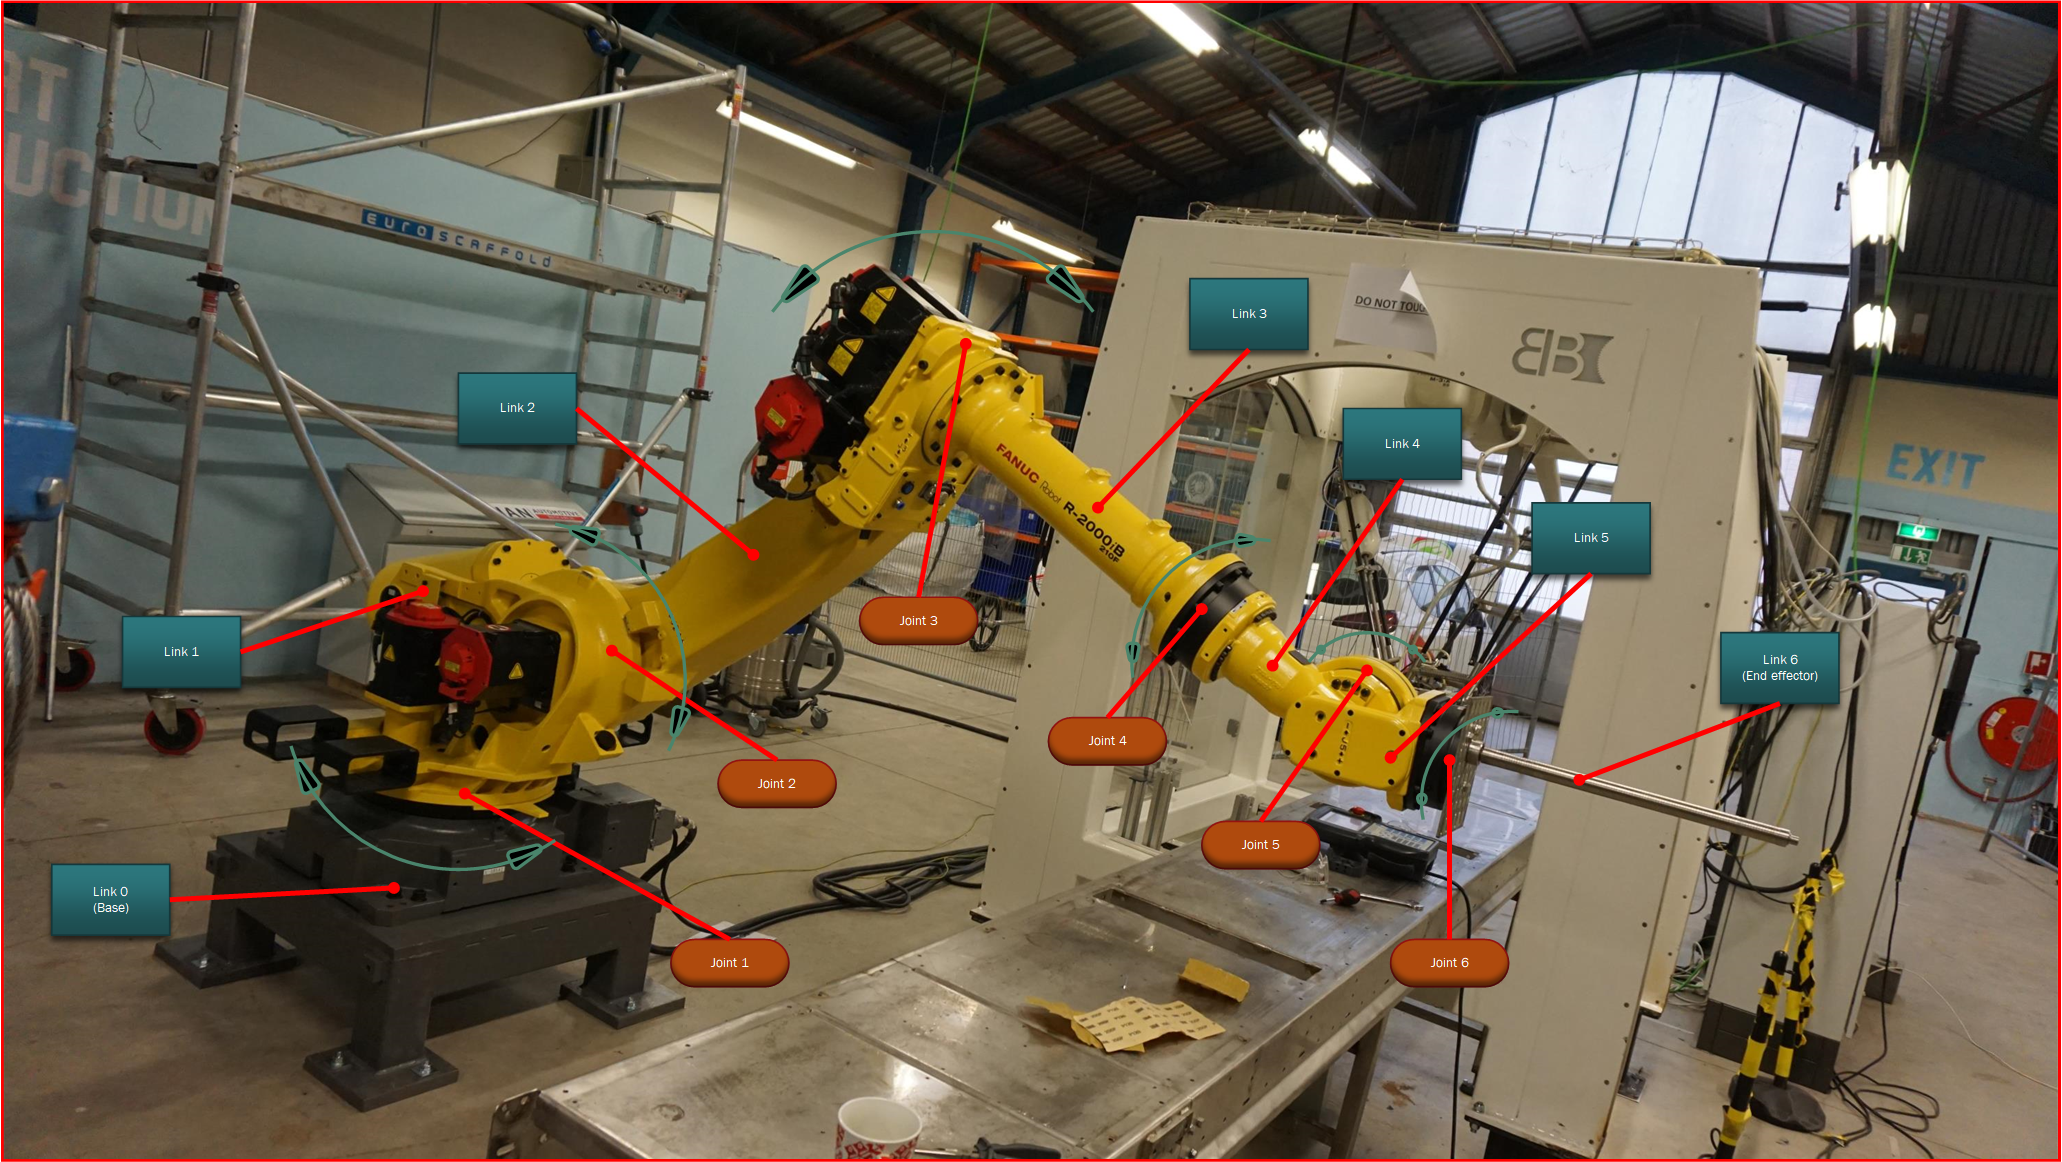
\includegraphics[
	width=1\linewidth,
	center,
	keepaspectratio,
	]{linksANDjoints/linksAndJoints}
	\caption{Links (turquoise) and joints (orange) in the FANUC 210F}
	\label{fig:LinksANDJoints210F}
\end{figure}

\paragraph{\textbf{\gls{z_i}} axes in Fanuc 210F}
As described in \fullref{par:z_iAxesAssign}, the $\gls{z_i}$ axes can be attached to the Fanuc 210F (see figure \ref{fig:zi_Axes}).


\begin{figure}[H]
	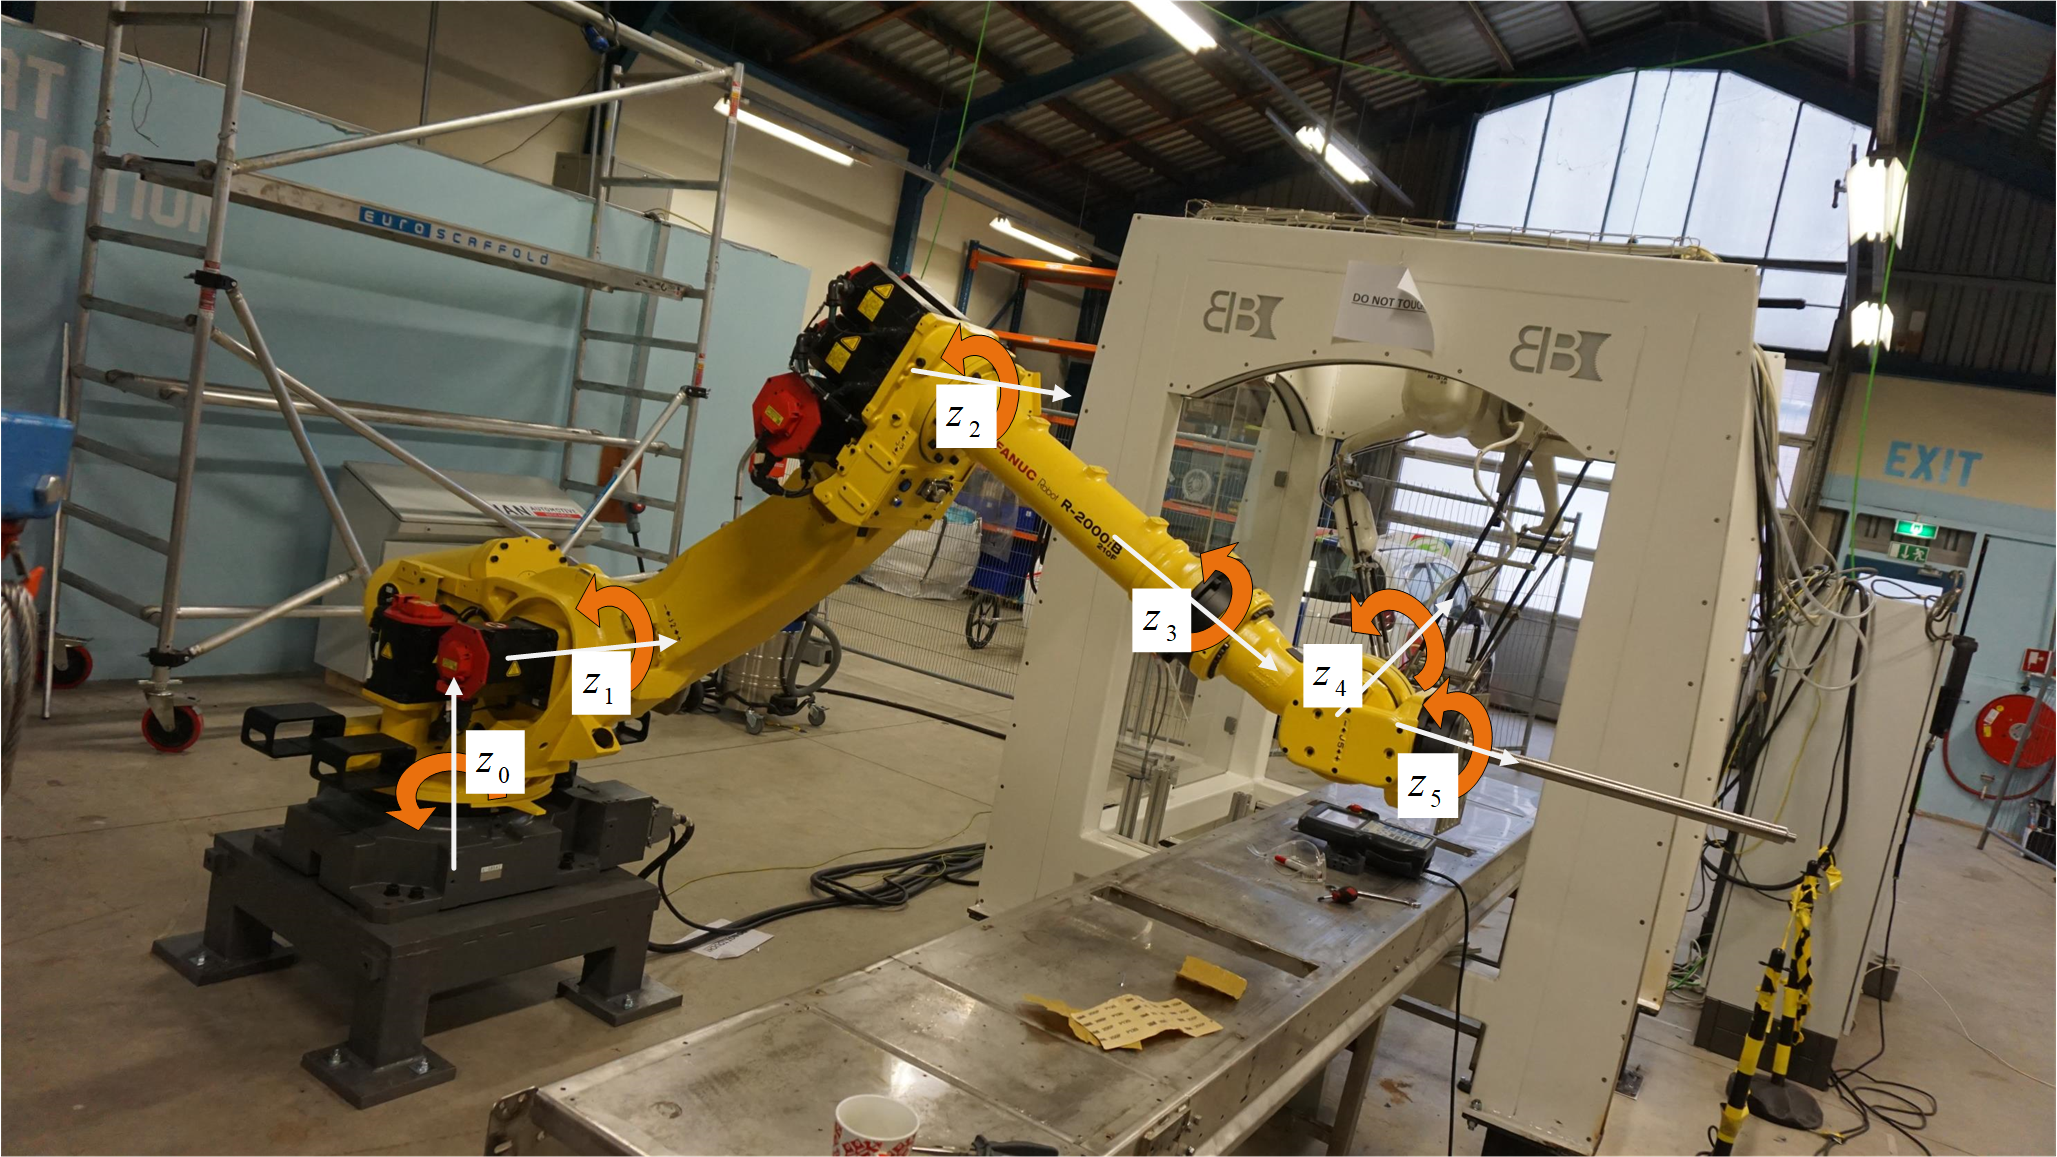
\includegraphics[
	width=1\linewidth,
	center,
	keepaspectratio,
	]{coordinateFrames/z_axes}
	\caption{$z_i$ axes on the Fanuc 210F with the direction of positive rotation (orange)}
	\label{fig:zi_Axes}
\end{figure}


The positive direction of the triples $z_1$, $z_2$, $z_4$ and $z_0$, $z_3$, $z_5$, was chosen to make sure, the x-axis would always have the same direction for parallel joints. 

\subsubsection{local coordinate reference frames on the Fanuc 210F}

As described in \fullref{sec:localRefFrame}, the local coordinate reference frames can also be attached to the Fanuc 210F as seen in figure \ref{fig:RefFrame}. 

\begin{figure}[H]
	\includegraphics[
	width=1\linewidth,
	center,
	keepaspectratio,
	]{coordinateFrames/CoordinateFramesRobotStandardPose}
	\caption{Coordinate reference frames for Fanuc 210F in standard (Normal) pose}
	\label{fig:RefFrame}
\end{figure}


\paragraph{Abstract view of coordinate frames}
For a better overview, the drawing of the robot can be removed, which reveals the pure coordinate frames. In figure \ref{fig:RefFrameAbstract} is described, in which relation the coordinate frames stand to each other.

\begin{figure}[H]
	\includegraphics[
	width=1\linewidth,
	center,
	keepaspectratio,
	]{coordinateFrames/CoordinateFrames}
	\caption{Coordinate reference frames for Fanuc 210F}
	\label{fig:RefFrameAbstract}
\end{figure}

\paragraph{assignment of indvidual frames}
The assignment of individual frames can be found in appendix \fullref{app:IndFrameAss}





\subsubsection{Establishing \ac{DH} parameters on the Fanuc 210F}

As described in \fullref{sec:DHparPerLink}, the \ac{DH}-Parameters can also be determined for the Fanuc 210F.
These parameters can be found with the help of the assigned coordinate frames as seen in figure \ref{fig:DH_Parameters_Fanuc210F}. For simplicity, only non-zero DH-parameters are shown in this figure.

\begin{figure}[H]
	\includegraphics[
	width=1\linewidth,
	center,
	keepaspectratio,
	]{coordinateFrames/DH_Parameters_assignment}
	\caption{Assignment of DH-Parameters on the Fanuc 210F}
	\label{fig:DH_Parameters_Fanuc210F}
\end{figure}


To wrap this up, a summary of the D-H parameters for each link as follows from figure \ref{fig:DH_Parameters_Fanuc210F} can be found in table \ref{table:DH-Parameter}


%Generate tables easily with: % https://www.tablesgenerator.com/

\begin{table}[H]
	\centering
	\begin{tabular*}{0.5\textwidth}{|l||@{\extracolsep{\fill}}l|l|l|l|}
		\hline
		Link & \multicolumn{1}{l|}{$\theta_i$} & \multicolumn{1}{l|}{$d_i$} & \multicolumn{1}{l|}{$a_i$} & \multicolumn{1}{l|}{$\alpha_i$} \\ \hline\hline
		1 & $\theta_1$ & $d_1$ & $a_1$ & $\alpha_1$\\ \cline{1-5}
		2 & $\theta_2$ & 0     & $a_2$ & 0         \\ \cline{1-5}
		3 & $\theta_3$ & 0     & $a_3$ & $\alpha_3$\\ \cline{1-5}
		4 & $\theta_4$ & $d_4$ & 0     & $\alpha_4$\\ \cline{1-5}
		5 & $\theta_5$ & 0     & 0     & $\alpha_5$\\ \cline{1-5}
		6 & $\theta_6$ & $d_6$ & 0     & 0         \\ \cline{1-5}
		%\hline
	\end{tabular*}
	\caption{\acrfull{DH} Parameters for Fanuc 210F}
	\label{table:DH-Parameter}
\end{table}


\paragraph{numeric values of DH-Parameters}

As can be seen from table \ref{table:DH-Parameter}, many \ac{DH}-parameters are zero due to a good choice of pose and coordinate frames. 
All angles are plus or minus 90°.

Most of the frames have translational transformations in either $\gls{a_i}$ or $\gls{d_i}$ direction with link 1 and 5 being the exception.
By lifting the base frame out of the joint, parameter $d_1$ could be set to zero as well. For better understanding, the origin of the frame was originally kept inside the joint.
Frame 5 shares the origin with frame 4, not requiring any translational movement.
Most of the frames are also rotated by 90 degree around the x-axis with link 2 and 6 being the exception. Frame 6 was chosen with the same orientation as frame 5. Frame 2 has the same x-axis orientation as link 1 because joints two and three are parallel. There is just a rotational transformation around the z-axis of 90°. This is only due to the standard pose of the robot, as theta is a variable.
For all coordinate frames theta is a variable, as all joints are revolute and none is translational. 

Besides the angle values for $\alpha_i$ which were easy to determine from the graphical interpretation in figure \ref{fig:DH_Parameters_Fanuc210F}, following numeric values need to be determined through measurements or CAD-Drawings:
$d_1$, $d_4$, $d_6$ and \\
$a_1$, $a_2$, $a_3$. 

A great help to determine these values is fig \ref{fig:RefFrame}. This technical drawing was obtained from the data-sheet for all Fanuc R-2000iB series robots. 
With this drawing, following \ac{DH}-parameters can be obtained:

\begin{itemize}\label{item:DH-LinparamValues}
	\item[$a_1$=] 312 [\textit{mm}]
	\item[$a_2$=] 1075 [\textit{mm}]
	\item[$a_3$=] 225 [\textit{mm}]
	\item[$d_4$=] 1280 [\textit{mm}]
	\item[$d_6$=] 235 [\textit{mm}]
\end{itemize}

The parameter $d_1$ cannot be determined from this drawing. It can either be measured on the actual robot, or defined as zero, as frame zero can be freely moved along the z-axis. A value of zero would put the origin of the base frame on the same height as frame 1, simplifying subsequent steps. 
It must be clear though, that all referencing in the forward and backward kinematics will be relative to this point. 
A change of this point of reference can be added later simply by adding another transformation matrix for translational movement along the z-axis as presented by Richard P. Paul \cite{Paul1981RobotM}.\\
\\
This results in a table of numeric DH-parameters as seen in \ref{table:DH-Parameter_num}. The transformation $^{i-1}T_i$ depends only on a single variable $\gls{theta_i}$ as all of the other quantities stay constant, and all joints are revolute.

\begin{table}[H]
	\centering
	\begin{tabular*}{0.5\textwidth}{|l||@{\extracolsep{\fill}}l|l|l|l|}
		\hline
		Link & \multicolumn{1}{l|}{$\theta_i$} & \multicolumn{1}{l|}{$d_i$} & \multicolumn{1}{l|}{$a_i$} & \multicolumn{1}{l|}{$\alpha_i$} \\ \hline\hline
		1 & $\theta_1$ & 0     & 312   & $\pi/2$  \\ \cline{1-5}
		2 & $\theta_2$ & 0     & 1075  & 0        \\ \cline{1-5}
		3 & $\theta_3$ & 0     & 225   & $\pi/2$  \\ \cline{1-5}
		4 & $\theta_4$ & 1280  & 0     & $-\pi/2$ \\ \cline{1-5}
		5 & $\theta_5$ & 0     & 0     & $\pi/2$  \\ \cline{1-5}
		6 & $\theta_6$ & 235   & 0     & 0        \\ \cline{1-5}
		%\hline
	\end{tabular*}
	\caption{Numeric values of Denavit Hartenberg Parameters for Fanuc 210F}
	\label{table:DH-Parameter_num}
\end{table}


\subsubsection{Calculate homogeneous transformation matrices}

For further details on how to set up $R_z(\theta_i), T_z(d_i), T_x(a_i) and R_x(\alpha_i)$ and form the transformation matrix in equation \ref{eq:TransformationMarix} see chapter 1 "Homogeneous Transformations" in %"Robot manipulators: mathematics, programming, 
and control: the computer control of robot manipulators" 
\cite{Paul1981RobotM}. The basic techniques for setting up the translation and rotation matrices as well as how to combine them are described in that chapter .




\subsubsection{Forward Kinematic Equations on the 210F}
As shown in fig.\ref{fig:zi_Axes}, the Fanuc 210F is a 6-\ac{DOF} robotic arm with \gls{N}=six revolute joints in series. 
Their orientation can be expressed in short form with 
\begin{equation}
(R\perp R\parallel R\perp R\perp R\perp R )
\end{equation}

With this, the complete transformation matrix can be derived in the form as described in \ref{ForKinEq}:

%\begin{equation}
\begin{multline}\label{eq:TransformMatrices_0-6}
	^0T_6=\\
	\begin{bmatrix}
\cos\theta_1 & -\sin\theta_1 \cdot \cos\alpha_1 & \sin\theta_1 \cdot \sin\alpha_1 & a_1 \cdot \cos\theta_1 \\
\sin\theta_1 & \cos\theta_1 \cdot \cos\alpha_1 & -\cos\theta_1 \cdot \sin\alpha_1 & a_1 \cdot \sin\theta_1 \\
0 & \sin\alpha_1 & \cos\alpha_1 & d_1 \\
0 & 0 & 0 & 1 \\
\end{bmatrix}
 \cdot \\
\begin{bmatrix}
\cos\theta_2 & -\sin\theta_2 \cdot \cos\alpha_2 & \sin\theta_2 \cdot \sin\alpha_2 & a_2 \cdot \cos\theta_2 \\
\sin\theta_2 & \cos\theta_2 \cdot \cos\alpha_2 & -\cos\theta_2 \cdot \sin\alpha_2 & a_2 \cdot \sin\theta_2 \\
0 & \sin\alpha_2 & \cos\alpha_2 & d_2 \\
0 & 0 & 0 & 1 \\
\end{bmatrix}
 \cdot \\
\begin{bmatrix}
\cos\theta_3 & -\sin\theta_3 \cdot \cos\alpha_3 & \sin\theta_3 \cdot \sin\alpha_3 & a_3 \cdot \cos\theta_3 \\
\sin\theta_3 & \cos\theta_3 \cdot \cos\alpha_3 & -\cos\theta_3 \cdot \sin\alpha_3 & a_3 \cdot \sin\theta_3 \\
0 & \sin\alpha_3 & \cos\alpha_3 & d_3 \\
0 & 0 & 0 & 1 \\
\end{bmatrix}
 \cdot \\
\begin{bmatrix}
\cos\theta_4 & -\sin\theta_4 \cdot \cos\alpha_4 & \sin\theta_4 \cdot \sin\alpha_4 & a_4 \cdot \cos\theta_4 \\
\sin\theta_4 & \cos\theta_4 \cdot \cos\alpha_4 & -\cos\theta_4 \cdot \sin\alpha_4 & a_4 \cdot \sin\theta_4 \\
0 & \sin\alpha_4 & \cos\alpha_4 & d_4 \\
0 & 0 & 0 & 1 \\
\end{bmatrix}
 \cdot \\
\begin{bmatrix}
\cos\theta_5 & -\sin\theta_5 \cdot \cos\alpha_5 & \sin\theta_5 \cdot \sin\alpha_5 & a_5 \cdot \cos\theta_5 \\
\sin\theta_5 & \cos\theta_5 \cdot \cos\alpha_5 & -\cos\theta_5 \cdot \sin\alpha_5 & a_5 \cdot \sin\theta_5 \\
0 & \sin\alpha_5 & \cos\alpha_5 & d_5 \\
0 & 0 & 0 & 1 \\
\end{bmatrix}
 \cdot \\
\begin{bmatrix}
\cos\theta_6 & -\sin\theta_6 \cdot \cos\alpha_6 & \sin\theta_6 \cdot \sin\alpha_6 & a_6 \cdot \cos\theta_6 \\
\sin\theta_6 & \cos\theta_6 \cdot \cos\alpha_6 & -\cos\theta_6 \cdot \sin\alpha_6 & a_6 \cdot \sin\theta_6 \\
0 & \sin\alpha_6 & \cos\alpha_6 & d_6 \\
0 & 0 & 0 & 1 \\
\end{bmatrix}
\phantom{ \cdot }\\
\end{multline}
%\end{equation}

This set of matrices can be filled with the numerical values from table \ref{table:DH-Parameter_num}. The intermediate steps, that lead to the forward kinematic equations, can be found in appendix \fullref{sec:FWKinEqSteps}


With matrix \ref{eq:matrixForm}, the forward kinematic equations can be formed:

\begin{dmath}\label{eq:ForwardKinEquations_6DOF}
	n_x = \\ \cos\theta_1(\cos(\theta_2+\theta_3)(\cos\theta_4\cos\theta_5\cos\theta_6-\sin\theta_4\sin\theta_6)-\sin(\theta_2+\theta_3)\sin\theta_5\cos\theta_6)+\sin\theta_1(\sin\theta_4\cos\theta_5\cos\theta_6-\cos\theta_4\sin\theta_6)\\
	n_y = \\ \sin\theta_1(\cos(\theta_2+\theta_3)(\cos\theta_4\cos\theta_5\cos\theta_6-\sin\theta_4\sin\theta_6)-\sin(\theta_2+\theta_3)\sin\theta_5\cos\theta_6)-\cos\theta_1(\sin\theta_4\cos\theta_5\cos\theta_6-\cos\theta_4\sin\theta_6) \\
	n_z = \\ \sin(\theta_2+\theta_3)(\cos\theta_4\cos\theta_5\cos\theta_6-\sin\theta_4\sin\theta_6)-\cos(\theta_2+\theta_3)\sin\theta_5\cos\theta_6 \\
	o_x = \\ \cos\theta_1(-\cos(\theta_2+\theta_3)(\cos\theta_4\cos\theta_5\sin\theta_6+\sin\theta_4\cos\theta_6)-\sin(\theta_2+\theta_3)\sin\theta_5\sin\theta_6)-\sin\theta_1(\sin\theta_4\cos\theta_5\sin\theta_6-\cos\theta_4\sin\theta_6) \\
	o_y = \\ \sin\theta_1(-\cos(\theta_2+\theta_3)(\cos\theta_4\cos\theta_5\sin\theta_6+\sin\theta_4\cos\theta_6)-\sin(\theta_2+\theta_3)\sin\theta_5\sin\theta_6)+\cos\theta_1(\sin\theta_4\cos\theta_5\sin\theta_6-\cos\theta_4\sin\theta_6) \\
	o_z = \\ -\sin(\theta_2+\theta_3)(\cos\theta_4\cos\theta_5\sin\theta_6+\sin\theta_4\sin\theta_6)-\cos(\theta_2+\theta_3)\sin\theta_5\sin\theta_6 \\
	a_x = \\ \cos\theta_1(\cos(\theta_2+\theta_3)\cos\theta_4\sin\theta_5+\sin(\theta2+\theta_3)\cos\theta_5)+\sin\theta_1\sin\theta_4\sin\theta_5 \\
	a_y = \\ \sin\theta_1(\cos(\theta_2+\theta_3)\cos\theta_4\sin\theta_5+\sin(\theta2+\theta_3)\cos\theta_5)+\cos\theta_1\sin\theta_4\sin\theta_5 \\
	a_z = \\ \sin(\theta_2+\theta_3)\cos\theta_4\sin\theta_5-\cos(\theta_+\theta_3)\cos\theta_5 \\
	p_x = \\
	\cos\theta_1(a_1+a_2\cos\theta_2+a_3\cos(\theta_2+\theta_3)+d_4\sin(\theta_2+\theta_3)+d_6(\cos(\theta_2+\theta_3)\cos\theta_4\sin\theta_5+\sin(\theta_2+\theta_3)\cos\theta_5))+d_6\sin\theta_1\sin\theta_4\sin\theta_5 \\
	p_y = \\
	\sin\theta_1(a_1+a_2\cos\theta_2+a_3\cos(\theta_2+\theta_3)+d_4\sin(\theta_2+\theta_3)+d_6(\cos(\theta_2+\theta_3)\cos\theta_4\sin\theta_5+\sin(\theta_2+\theta_3)\cos\theta_5))+d_6\sin\theta_1\sin\theta_4\sin\theta_5 \\
	p_z = \\
	a_2\sin\theta_2+a_3\sin(\theta_2+\theta_3)-d_4\cos(\theta2+\theta_3)+d_6(\sin(\theta_2+\theta_3)\cos\theta_4\sin\theta_5-\cos(\theta_2+\theta_3)\cos\theta_5) \\
\end{dmath}

In these equations, the numerical values were replaced with their parameter name. These numeric values can be found in section \ref{item:DH-LinparamValues}.


These kinematic equations can be used to simulate the movements of a robot with given angle-values for the joints. 















	\chapter{Inverse Kinematics}

With the forward kinematic equations, the position of the end effector can be determined relative to the base frame for given values of the joint variables.
In the context of robotics, it is also necessary to determine these joint variables for a given end effector position.
This is referred to as the inverse kinematic problem.
Solving the inverse kinematic problem for a given serial link actuator allows to transform a motion plan of the \ac{EOAT} into joint actuator trajectories for the robot.\\
\\
\section{Existance of solutions}
A 6\ac{DOF} robot has multiple sets of inverse solutions. As stated by YanWu et al. there are 8 groups of inverse solution for most \ac{EOAT}-positions within the manipulator's workspace \cite{invKinSolYanWu}. 
Not all positions are equally reachable though.
There are two types of workspace:
\begin{itemize}
	\item[Dextrous workspace] volume of space that the robot end-effector can reach with all orientations
	\item[reachable workspace] volume of space, that the robot can reach in at least one orientation
\end{itemize}
\cite{craig1986introduction}
A manipulator with less than 6\ac{DOF} cannot reach all positions and orientations in 3D-space. 

%https://robotics.stackexchange.com/questions/10322/is-it-possible-to-get-all-possible-solutions-of-inverse-kinematics-of-a-6-dof-ar
%In general, if the wrist is spherical (i.e., all three axes intersect), you can enumerate all of the various closed-form solutions through a method known as wrist partitioning. This method uses the three arm joints to solve for the position of the wrist center. It then uses the wrist joints to determine the joint angles which orient the end effector properly. Multiple solutions are possible from "wrist up" and "wrist down" options, "elbow up" and "elbow down" options (for an articulated arm), and "over the shoulder" options also. For other robot geometries the options would differ.

%If the wrist is not spherical, it becomes quite challenging to find a closed-form inverse solution. But you still have the various geometric options for inverse kinematics solutions.
%
%One way to make sure you are identifying all of the solutions is to recall the fundamentals of trigonometry. Recall that sin(θ)=−sin(−θ)
%and cos(θ)=cos(−θ). So when you are solving for θ you have to consider the other angles which produce the same result using these and other trigonometric identities. 
	\chapter{\ac{DH}-Convention} \label{sec:DH-convention}

The \ac{DH}-Convention is a commonly used and simplifies the forward and backward transformation. It was named after Jaques Denavit and Richard Hartenberg who developed a general theory to describe a serial link mechanism. \cite{DenavitHartenbergLesson}\\
It consists of following parts:

\begin{itemize}[leftmargin=3cm]
	\item \ac{DH}-Convention for establishing the coordinate systems
	\item \ac{DH}-Transformation for generation of the coordinate systems
	\item \ac{DH}-Parameters as a result form the transformations
\end{itemize}

Determining the coordinate systems is done according to set rules. Nevertheless, the choices of coordinate frames are also not unique, so different people will derive different, but correct frame assignments. This freedom of choice should be used to bring as many \ac{DH}-Parameters as possible to zero. This simplifies subsequent equations and calculations. \cite{DenavitHartenbergKonventionen}

Each joint of the robot is described by four parameters.

This leads to a kinematic chain with each frame determined by the previous one \cite{DenavitHartenbergKonventionen}.\\
\\

Link0 - Link1 - Link2 - Link3 - Link4 - Link5 - Link6\\
\\

Each \ac{DH}-transformation consists of four elementary transformations \cite{DenavitHartenbergKonventionen}:

\begin{enumerate}[label=\emph{\arabic*)}]
	\item rotation around the $x_i$-axis with the amount of $\alpha_i$
	\item translation along $x_i$-axis with the amount of  $a_i$
	\item translation along $z_i$-axis with the amount of  $d_i$
	\item rotation around $z_i$-axis with the amount of  $\theta_i$
\end{enumerate}

A definition of these base transformations is given in  \cite{allgInvKin}, Section 2.1.

This shows that the \ac{DH} robotic convention is a minimal line representation, as with four parameters, all possible lines in the Euclidean Space can be represented (\cite{AutRobVeh}, page 210).

Following from this, two pairs of parameters determine the joints and links \cite{ConstantinForwardKA}:
\begin{itemize}[wide=\parindent] 
	\item[Links:] represented by link length ($a$) and link twist ($\alpha$)
	%, defined as the relative location of the two attached joint axes.
	\item[Joints:] represented by link offset ($d$)
	% which is the distance from one link to the next 
	and joint angle ($\theta$) 
	%which is the rotation of one link with respect to the next around the joint axis.
\end{itemize}
\phantom{}\\

	
%	\input{ThesisWork/}
	
	
	\section{Robot configurations}

As mentioned before, a 6 \ac{DOF} manipulator can reach the same position in multiple configurations.
The different configurations in the solutions can be seen in the example of the FANUC robot arms (see figure \ref{fig:RobotConfigs})
\medskip
%\begin{itemize}
%	\item Flip vs. No-Flip
%	\item Up vs. Down
%	\item Front vs. Back
%\end{itemize} \cite{OneRobFanucConfigurations}

\begin{figure}[H]
	\includegraphics[
	width=0.6\linewidth,
	center,
	keepaspectratio,
	]{FanuRobotConfigurations_cr}
	\caption{6 axis robot configurations on the example of a FANUC Robot \cite{QingFanucAcademy}}
	\label{fig:RobotConfigs}
\end{figure}
	

	\renewcommand{\bibname}{References}
	\printbibliography
	\newpage
	
	
	\begin{appendices}
		\input{Appendices/Appendix1}
		\input{Appendices/Appendix2}
		%\chapter{Choice of IP address space}

%\url{https://en.wikipedia.org/wiki/Private_network}
 
It is in the class B of private IPv4 address space. Usually for home networks class c networks $ (192.168.0.0 – 192.168.255.255) $ are used. These allow to address$  256 $ adresses per subnet. without the gateway$  (.0) $ the broadcast address $ (.255) $ and an address for the router, we're left with 253 addresses. 
For the beginning, it might be an address space that is big enough, but if we include a lot of sensors, and other things, a space of 253 addresses might get small. 
 
Also this address space is usually used with a subnet mask of 255.255.0.0 which allows a mapping of  255 main addresses (172.x.0.x - 172.x.255.x) with 255 subpoints (172.x.x.0 - 172.x.x.255). Like this, each domain can get their own subnet (172.16.x.x-172.31.x.x), each device can get a main address space and then the different ports on the machines can be given numbers.
 
Also the  B block is not that commonly used, so this works also as a first line of defence against attachs from outside. Port knocking e.g. becomes harder, as the address space is way bigger.
		\chapter{Robot Quick start guide}
A big part of this was derived from \cite{MatlabControl}.

\paragraph{Parts of the robot}
A quick overview over the visible parts.

\subparagraph{FANUC R-2000iC/210F 6 axis robotic arm}
The robot has 6 movable joints with a possible payload attached to the end. Its features include a wide reach (2655 mm), sturdy but flexible arm design, a spring loaded counterbalance, relatively high payload capacity (210Kg) and fast moving axes. The joints also have hashes to indicate the zero positions which help with the calibration of the robot. 

\subparagraph{R30iA Robot Controller }
The Robot is controlled using an original equipment manufacturer controller called the FANUC R30iA controller. Its features include faster sustained speed and superior position accuracies. It also has the I/O ports that are used to connect grippers and other payloads. (It also houses the camera circuits which are required to access the data from the SONY camera provided with the robot. - Delta only)  The controller is also provided with a data card slot in which the special SD cards manufactured can be inserted and used as external memory. On the outside of the controller (side of iPendant at Delta) a USB port can be found. With these, programs, firmware files and other files can easily be transferred. Additionally, there is extended connectivity via its Ethernet port e.g. for FTP available.

\subparagraph{iPendant}
The teaching pendant is the primary user interface to the robot. It is used to move the joints of the robot manually, to program specific trajectories, to control the gripper, and various other actions. It also is an interface that can be used for input and output of the robot controller parameters. The user can access the system variables and position variables. (It is provided with a USB port that can be used to connect to a USB drive for external storage. - Delta only) It can also be used to setup an FTP server and client in order to communicate with the PC. 

\subparagraph{Gripper}
The robot as handed over does not have an active gripper system. It has been tested though with a pneumatic gripper controlled via the DO ports and pneumatic valves. A 2-way pneumatic valve, some piping and a pressure regulator are still available. (Delta Equipment varies here a lot).


\paragraph{iPendant Navigation Manual:}
The teaching pendant is the primary user interface to the robot. This section deals with the important 
buttons on the TP. 


\begin{figure}[H]
	\centering
	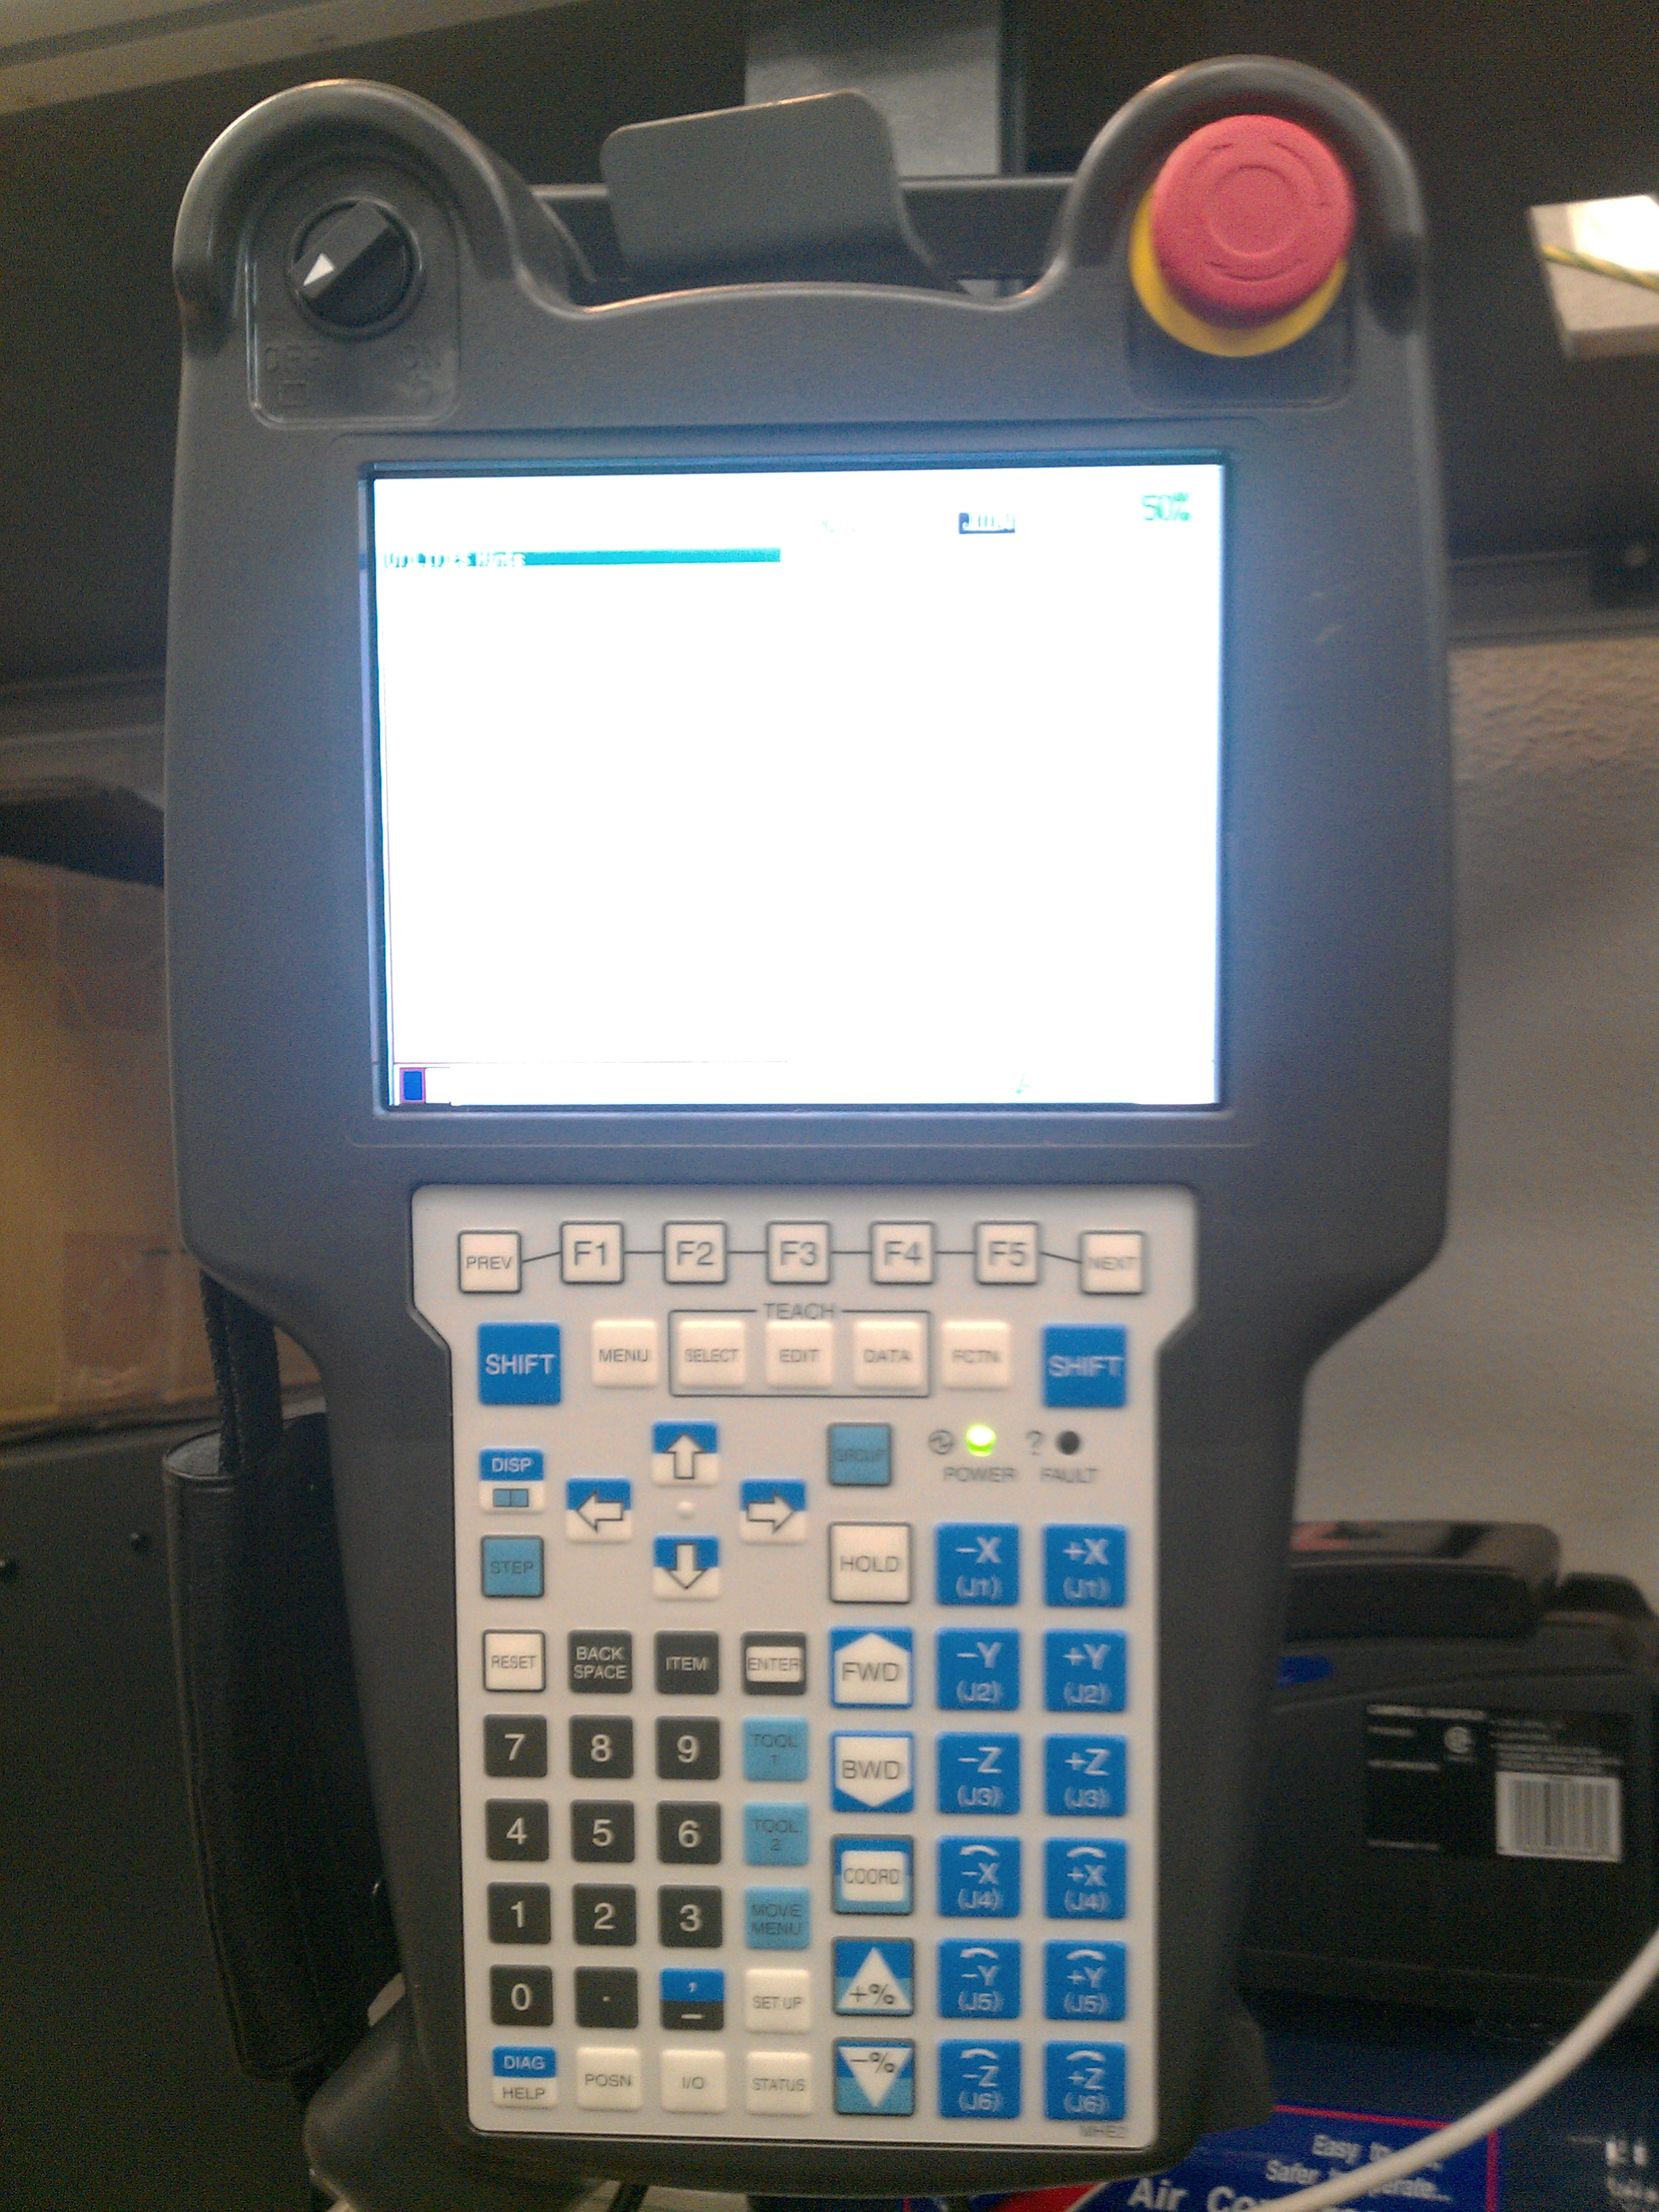
\includegraphics
	[width=0.8\linewidth
	]{images/iPendant_Numbered}
	\caption[Important buttons]{Most important iPendant buttons numbered: This image from another iPendant than the ones available was chosen because of its labelling of buttons. Some buttons of the available iPendants are not labelled, so this picture can be used as a reference. Source: \cite{MatlabControl}}
	\label{fig:ipendantnumbered}
\end{figure}


\subparagraph{Emergency stop: }

Makes the robot stop immediately by applying brakes. Use it only when necessary as the brakes wear down. There is also an E-stop on the controller.
Press down on the button to activate it.
Twist it to the right to release.
If a slow and gradual halt is required, press HOLD on the iPendant.
TP on/off:
Below the E-stop button. It should be ON to access any function in the Teach Pendant (Set-ups, calibration, programs etc) and OFF when running in AUTO mode.
Deadman switch
The 2 yellow bars behind the iPendant. 3 modes are available: Fully released, halfway pressed, fully pressed. Only the middle mode activates control.







		%\newpage
\chapter{IOT Projects:}

The \ac{SPC} is a research lab, that is in constant development to show the latest innovations and bring them to use in industrial applications.
In the context of the master-thesis "Using FANUC R-2000iC/210F (6-axis robot) for improved efficiency in FRC parts formation" the topic of digital twinning and with that \ac{IOT} has become a major research point. 
In order to bring the \ac{FRC} production line to its full potential, several new projects could be defined. 
These projects improve comfort, energy-efficiency, ease of use and safety of the lab.
Each of these projects is designed to provide a flexible workload for 1-3 students with varying results depending on the students experience level and semester. In case 3 students sign up for a project, the diligence work is expected to be fulfilled. Each student is expected to pick their own range of tasks that they fulfil.
Following project ideas are proposed:\\
\bigskip
%
\section*{Room Temperature Control System}

	\begin{figure}[H]
	\centering
	\includegraphics[
	width=0.5\linewidth,
	height=\paperheight,
	keepaspectratio,
	]{RoomTemp}
	\caption{Heating when noone needs it is waste! \cite{RoomTemp}}
	\label{fig: RoomTemp}
\end{figure}


The Lab of the \ac{SPC} has an old heating system controlled with electromechanical thermostats. 
Originally this system was designed to work with steam delivered by the \ac{IPKW}. 
Later this System was retrofitted with two gas heaters that have no feedback about the actual heating demand. This needs to be improved for comfort and energy-efficiency.\\
\\
Your assignment will be to replace the old and manual control with an open-source home automation system. That means choosing sensors, actuators, electronic components and clients as well as the type of home automation servers. 
A possible approach would be using thermocouples as sensors, transistors to switch the inputs of the heating system, using an ESP8266 for sensing and controlling with \ac{FHEM} as the underlying home automation server running on a raspberry pi.\\
diligence work: also include other room thermostats in the offices as well as lights\\
\\
Why are you the right one for this project? (Not all is required, but some should resonate with you)
\begin{itemize}
\item You are interested in automation systems
\item You like improving existing systems with electronics
\item You have experience with Arduino/ESP8266
\item You are not afraid to learn a new programming language to do some basic tasks
\item You like Linux
\item You like it warm and cozy in the morning :)
\end{itemize}
\bigskip
%
\section*{NFC based Machine Access}

	\begin{figure}[H]
	\centering
	\includegraphics[
	width=0.5\linewidth,
	height=\paperheight,
	keepaspectratio,
	]{NFC}
	\caption{\ac{NFC} \cite{NFC}}
	\label{fig: NFC}
\end{figure}


The Lab of the \ac{SPC} has several heavy machines that move at high velocities, apply high pressures or create high temperatures. Because of these and other risks, a zoned safety system would make the lab a lot safer, as people would then stay in their assigned working zones while leaving work at other places unaffected. Also machine access needs to be restricted to the assigned student, while still leaving a traceable, temporarily restricted access to other users if necessary.\\
\\
Your assignment will be creating a \ac{NFC} card based zone and machine access. You can base this on an existing framework, or do it yourself. You will set up several \ac{NFC} readers with microcontrollers. These microcontrollers need to send a signal to a server that compares the access parameters delivered from the \ac{NFC}-card with a database that you set up. In case of a match, a signal is sent back to the Arduino, that switches a relay to open the gate. Additionally the Arduino should listen to other inputs in case a product cycle needs to be finished or additional requirements need to be fulfilled. Also there should be a signal sent back, when someone checks out of a safety zone. Machine access should have a timeout. Make a nice frontend to manage access.\\
diligence work: Make the communication between server and client hard to hack\\
\\
Why are you the right one for this project? (Not all is required, but some should resonate with you)
\begin{itemize}
\item You are interested in safety/security systems
\item You like to integrate something new into an ongoing project
\item You have experience with programming
\item You like microcontrollers
\item You can make a \ac{GUI}
\item (For diligence work: You like crypto)
\end{itemize}
\bigskip
%
%\section{Visual tool management system}
%In the lab of the \ac{SPC} many students use different tools like hammer, screwdrivers, wrenches etc. These tools get used throughout the day but rarely find their way back to their designated places (I'm also guilty of this). After spending a long time in the lab, many tools loose their designated storage places. It would be handy to take a photo of a tool and receive information about where to store it. Additionally, through the database the catalogue of available tools could be searched. \\
%\\
%Your assignment will be the creation of a program that can take a photo of a tool, recognize it and give out a description of its storage place with a photo. You will create a computer vision tool, probably based on machine learning to recognize the wide palette of tools in the lab.\\
%diligence work: Make it an android app\\
%\\
%Why are you the right one for this project? (Not all is required, but some should resonate with you)
%\begin{itemize}
%\item You are interested in image recognition
%\item You like to come up with something new
%\item You have experience with programming, ideally in Python
%\item (Diligence work: You would like to make an app)
%\item You don't like hardware
%\item You hate looking for stuff ;-)
%\end{itemize}
%\bigskip
%%
	\end{appendices}
	
	
	
\end{document}

%Questions for Report writing:Ton.ammerlaan@han.nl
